\chapter{DVCS beam-spin asymmetry extraction}

In the previous chapter, the events were filtered to select the ones which have 
one and only one good electron, and other good particles in coincidence with 
the electron. This chapter explains the procedure we used to extract the 
beam-spin asymmetry observable following this order: clean the DVCS data sample 
by choosing good run list, ensure the exclusivity of the selected events by 
imposing the conservation laws, subtract the background by combining data with 
simulation, and binning the identified DVCS events. This chapter contains also 
an estimation of the systematic uncertainty contribution from each source on 
the measured beam-spin asymmetry.

In the following, the selection procedures of the coherent DVCS events is 
detailed and generalized to the cases of incoherent DVCS, the coherent 
$\pi^{0}$, and the incoherent $\pi^{0}$ channels.    
  
\section{Coherent channel}
\subsection{Good run list}
In principle, with constant beam luminosity, target density and pressure, the 
event rate has to be constant over the experimental time. Due to the changes in 
the experimental conditions, such as changing a trigger in a detector, a slight 
shift in the beam position or a system failure somewhere, this rate changes. We 
minimize the effects of these changes on the reconstructed events by selecting 
the good runs. To this aim, we monitor the ratio of the number of the good 
tracks reconstructed in the RTPC to number of the detected good electrons in 
CLAS (<tpc/e>) as a function of run number. Furthermore, we also look at this 
ratio in the six sectors of CLAS, as they are independent of each other and 
their performances might be different. 

In this work, after the PID procedures, a run is considered good if:
\begin{itemize}
\item The integrated $<tpc/e>$ rate over the six sectors of CLAS is consistent 
   with the neighboring runs.
\item The six sectors show small fluctuations for each run. 
\end{itemize}    

Figure \ref{fig:tpc_over_e_Run_sec.png} shows the integrated and the 
sector-dependence of <tpc/e> for the individual runs. One notices a universal 
variation of this ratio over the three months of data taking. This can be 
attributed to changes in the RTPC. In particular, we had leaks in our gas 
system that appeared during the run. This probably caused gas contamination, 
changing the properties of the detector.



\begin{figure}[h!]
\hspace*{-0.3in}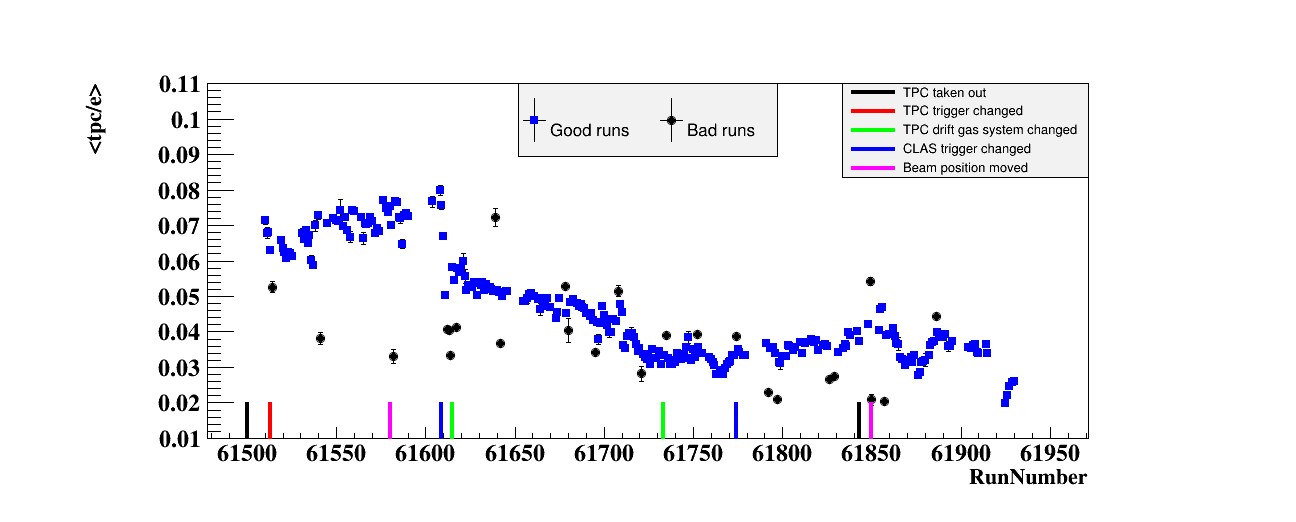
\includegraphics[scale=0.45]{fig_dvcs/tpc_over_e_Run.png}
\hspace*{-0.3in}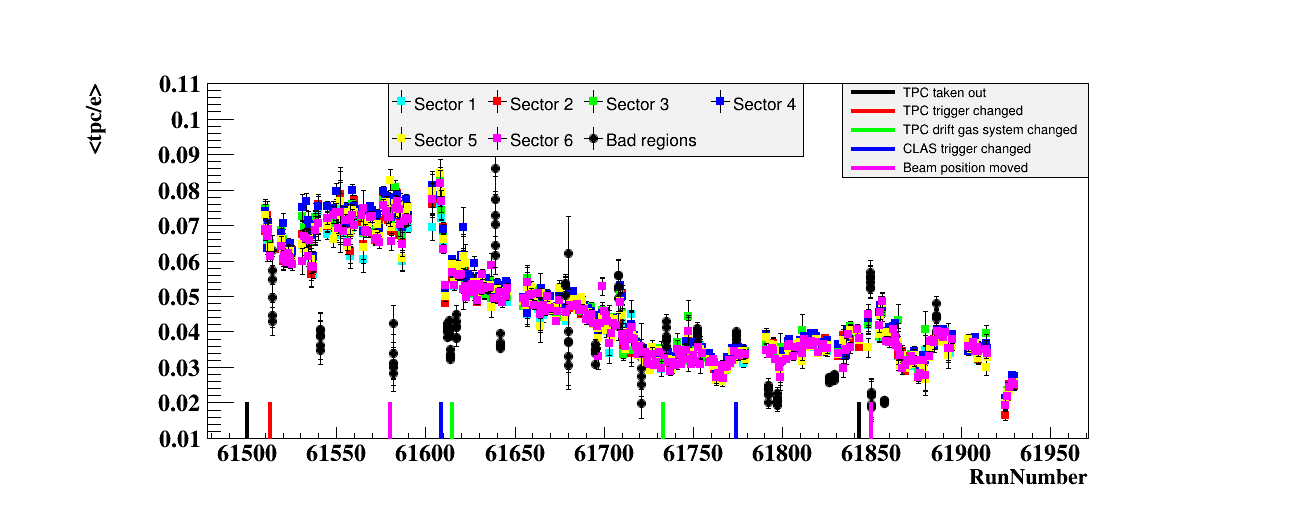
\includegraphics[scale=0.45]{fig_dvcs/tpc_over_e_Run_sec.png}
\caption{On the top: The integrated $<tpc/e>$ ratio (over the six sectors of 
   CLAS) for the individual runs. The blue points refer to the good runs, while 
   the black ones are the rejected ones. On the bottom: the $<tpc/e>$ ratio is 
   shown for each sector of CLAS. The colored points indicate the different 
   sectors for each good run, while the black ones are the rejected runs 
without color difference between the sectors. In both plots, the experimental 
setting changes that might cause a change in the event rate are indicated with 
vertical colored lines.} \label{fig:tpc_over_e_Run_sec.png}
\end{figure}

\subsection{Coherent DVCS event selection}
Events with one and only one good electron, one and only one good RTPC 
track and at least one good photon are considered good coherent DVCS 
candidates. Even though the DVCS reaction has only one real photon in the final 
state, events with more than one good photon are not discarded at this stage.  
This is motivated by the fact that some photons correspond to random 
coincidences and discarding these events results in losing good events. Then, 
events with one or more $\pi^{0}$ are removed from the coherent DVCS sample.  
After that, the most energetic photon in each remaining event is chosen as the 
DVCS photon. Next, to consider an event as a clean $^{4}He$ DVCS, it has to 
pass respectively two sets of requirements: DVCS characteristic cuts and 
exclusivity cuts.

~\newpage
\paragraph{DVCS characteristics}
\begin{itemize}
 \item $Q^{2}$ > 1 GeV$^{2}$: to ensure that the interaction occurs at the 
    partonic level and the applicability of the factorization in the DVCS  
    handbag diagram.
\item $ -t > -t_{min}$: the transferred momentum squared to the recoil $^{4}He$ 
   has to be greater than a minimum value defined by the kinematics of the beam 
   and the scattered electron as:
\begin{equation}
   t_{min} = - Q^{2} \frac{2(1- x_{A})(1 - \sqrt{1 + \epsilon ^{2}}) + \epsilon 
   ^{2}}{4 x_{A}(1-x_{A})+ \epsilon ^{2}},\\
\end{equation}
where $\epsilon ^{2} = \frac{4M^{2}_{^4He}x^{2}_{A}}{Q^{2}}$, $x_{A} = 
\frac{M_{p}\cdot x_{B}}{M_{^4He}}$ and $M_{p}$ ($M_{^4He}$) is the proton 
($^{4}He$) mass.

In the case of the proton DVCS, the variable $x_{A}$ is replaced by the Bjorken 
$x_{B}$ in the formula for $t_{min}$. Figure \ref{fig:tmin_both} presents 
$t_{min}$ distributions for both DVCS channels.

\item In the case of the incoherent DVCS channel, we apply a cut on the 
   invariant mass of the virtual photon and the target proton system to be
   greater than $2~GeV/c{^2}$. This cut avoids the region of excitation of the 
   proton to resonances.
 
\item $E_{\gamma}>$ 2 GeV. This is a cleaning cut applied to reduce the 
   background in the DVCS sample as the simulation indicates that no DVCS 
   events are expected with photon energy less than 2 GeV. Figure 
   \ref{fig:energy_dvcs_photons} shows the energy distributions of the 
   simulated coherent and incoherent DVCS events.

\begin{figure}[tbp]
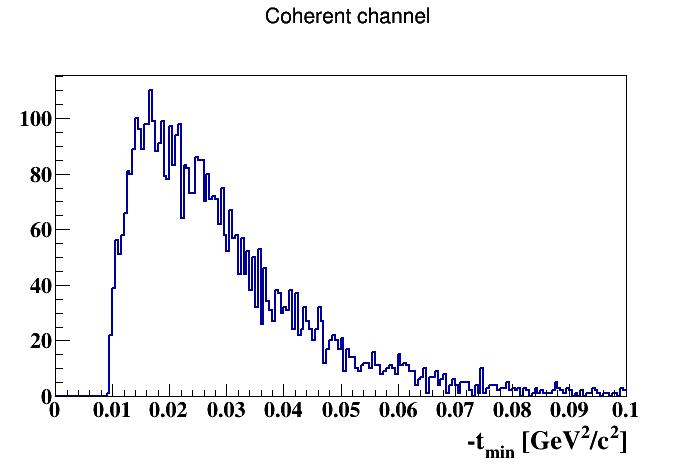
\includegraphics[height=5.0cm]{fig_rtpc/updates/tmin_coh.png}
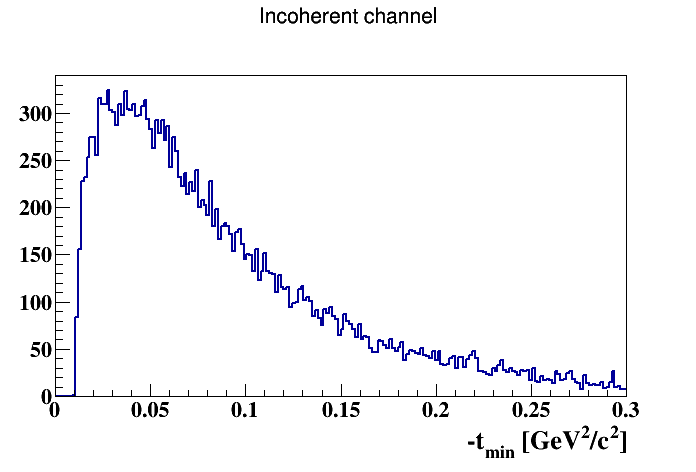
\includegraphics[height=5.0cm]{fig_rtpc/updates/tmin_incoh.png}
\caption{Coherent (left) and incoherent (right) -$t_{min}$ distributions 
calculated for the experimentally selected DVCS events. We use the experimental 
$Q^{2}$ and $x_{B}$ of the individual events. }
\label{fig:tmin_both}
 \end{figure}

\begin{figure}[tbp]
      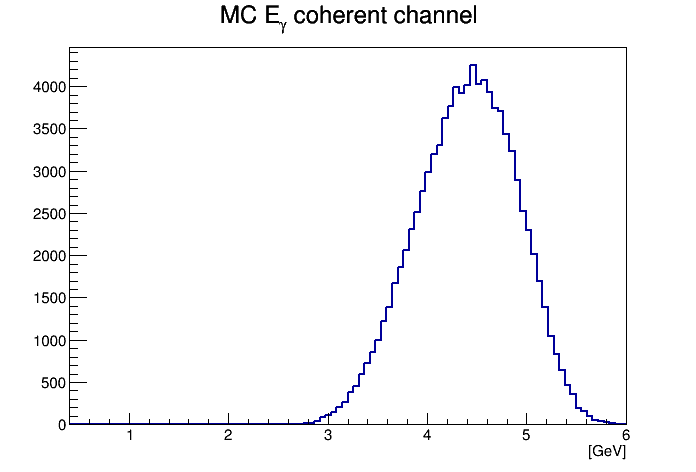
\includegraphics[height=5.0cm]{fig_dvcs/photon_energy_coh_sim.png}
      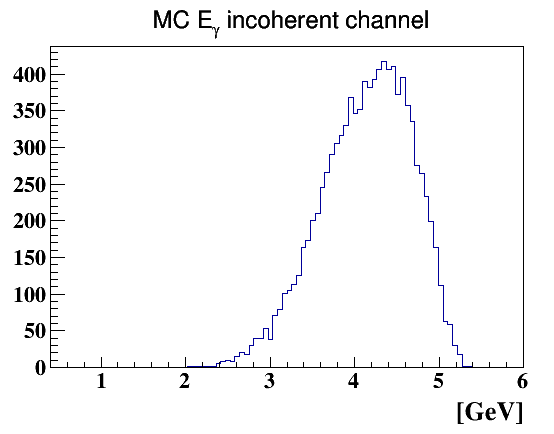
\includegraphics[height=5.5cm]{fig_dvcs/photon_energy_incoh_sim.png}
      \caption{The energy distribution of the simulated coherent (left) and 
      incoherent (right) DVCS photons.}
      \label{fig:energy_dvcs_photons}
\end{figure}
\end{itemize}

\newpage
\paragraph{Exclusivity cuts} ~\\
The coherent DVCS reaction is:
\begin{equation}
e(\mathbf{P}_{e}) + ~~^{4}He(\mathbf{P}_{^{4}He}) \rightarrow 
e'(\mathbf{P_{e'}}) +  ~~^{4}He'(\mathbf{P}_{^{4}He'}) + 
\gamma(\mathbf{P}_{\gamma})
\label{coh_dvcs_equ}
\end{equation}
where the symbols in the parentheses are the energy-momentum four-vectors. We define the additional four-vectors:
\begin{eqnarray}
\text{virtual photon vector } (\mathbf{P}_{\gamma^{*}}) &=&  \mathbf{P}_{e} -  \mathbf{P}_{e'} \\
\hspace{0.4in}  \mathbf{P}^{e^{4}He\gamma}_{X} &=& \mathbf{P}_{\gamma^{*}} + \mathbf{P}_{^{4}He} - (\mathbf{P}_{\gamma} + \mathbf{P}_{^{4}He'})\\
~~~~~~~~~~\mathbf{P}^{e^{4}He}_{X} &=& \mathbf{P}_{\gamma^{*}} + \mathbf{P}_{^{4}He} -  \mathbf{P}_{^{4}He'} \\
\hspace{0.2in} \mathbf{P}^{e\gamma}_{X} &=& \mathbf{P}_{\gamma^{*}} + \mathbf{P}_{^{4}He} - ~~\mathbf{P}_{\gamma}
\end{eqnarray}

The exclusivity of the coherent DVCS reaction is ensured by imposing the following conservation laws:
\begin{itemize}
\item The co-planarity cut ($\Delta \phi$). In principle, the virtual photon, the emitted real photon and the recoil helium lie in the same plane, which is called the hadronic plane. Thus the DVCS events must have $\Delta \phi$ values around zero. The hadronic plane can be defined in three ways:
\begin{eqnarray}
\overrightarrow{HP}_{1} &=& \overrightarrow{\mathbf{P}}_{^{4}He'} \times 
   \overrightarrow{\mathbf{P}}_{\gamma^{*}}\\
\overrightarrow{HP}_{2} &=& \overrightarrow{\mathbf{P}}_{^{4}He'}  \times 
   \overrightarrow{\mathbf{P}}_{\gamma}\\
\overrightarrow{HP}_{3} &=& \overrightarrow{\mathbf{P}}_{\gamma^{*}} \times 
   \overrightarrow{\mathbf{P}}_{\gamma}
\end{eqnarray}
$\Delta \phi$ is defined to be the $\phi$ difference between these planes and 
is calculable from three combinations: ($\overrightarrow{HP}_{1}$, 
$\overrightarrow{HP}_{2}$), ($\overrightarrow{HP}_{1}$, 
$\overrightarrow{HP}_{3}$) and ($\overrightarrow{HP}_{2}$, 
$\overrightarrow{HP}_{3}$). We investigated the three combinations and we 
decided to use the second one as it gives better resolution.

\item Missing energy, mass and transverse momentum ($p^{T}_{X} = 
   \sqrt{(p^{x}_{X})^2 + (p^{y}_{X}})^2$) cuts on 
   $\mathbf{P}^{e^{4}He\gamma}_{X}$.

\item Missing mass cuts on the $e^{4}HeX$ and $e\gamma X$ systems, which are 
   defined as $(P^{e^{4}He}_{X})^{2}$ and $(P^{e\gamma}_{X})^{2}$ respectively.

\item Cone angle cut between the measured real photon and the missing particle 
   in the $e^{4}HeX$ configuration. It is defined as:
\begin{equation}
\theta(\gamma, e^{4}HeX) = cos^{-1} \left( 
\frac{\overrightarrow{\mathbf{P}}_{\gamma} \cdot 
\overrightarrow{\mathbf{P}}^{e^{4}He}_{X}}{|\overrightarrow{\mathbf{P}}_{\gamma^{}}| 
|\overrightarrow{\mathbf{P}}^{e^{4}He}_{X}|}   \right).
\end{equation}
\end{itemize}
Figure \ref{fig:coh_exclusivty_cuts} summarizes all the exclusivity cuts.  In 
these plots, the black distributions represent the coherent events after the 
DVCS characteristic cuts and before all the exclusivity cuts. The shaded 
distributions stand for the events which passed all the exclusivity cuts except 
the one on the quantity plotted. We fitted each shaded distribution by a 
Gaussian and then we applied  3$\sigma$ cuts around the mean value of each 
distribution except the missing energy distribution for which a final 
[-0.45:0.5] GeV cut is applied to remove the tails and reduce the background.   
The events which pass these cuts are assumed to be good $^{4}He$ DVCS events. 

\begin{figure}[!h]
\centering
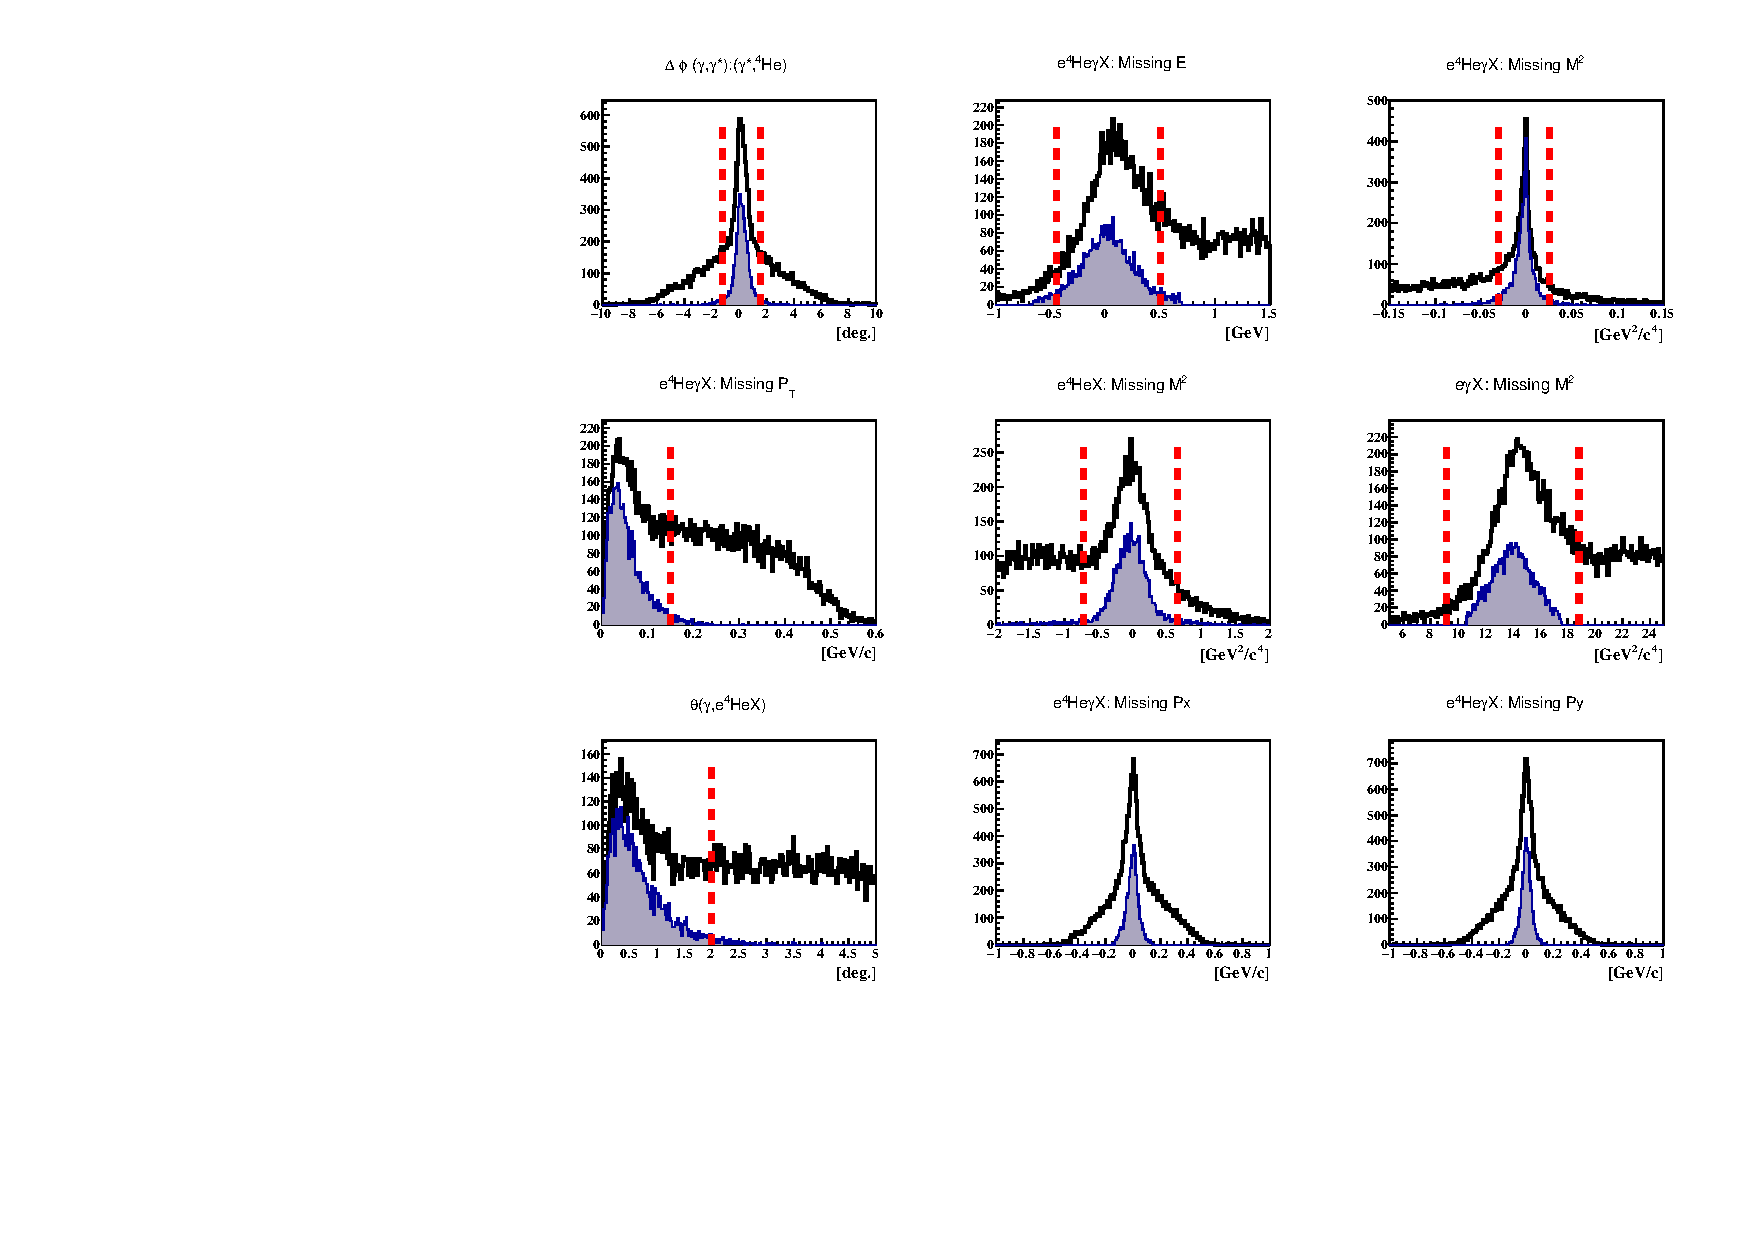
\includegraphics[scale=0.9]{fig_Dec2016/all_coh_exc_cuts.pdf}
\caption{The coherent DVCS exclusivity cuts. The blue distributions represent 
   the coherent DVCS events candidate. The shaded distributions represent the 
   events which passed all the exclusivity cuts except the quantity plotted.  
   The vertical red lines represent $3\sigma$ cuts on all the distribution 
   except the missing energy distribution for which [-0.45:0.5] GeV cut is 
   applied.  The missing momentum in $x$ and $y$ directions in the 
configuration $e^{4}He\gamma X$, are shown for information. The mean and the 
sigma values of each quantity can be found in Appendix \ref{exclusivity_cuts}, 
table \ref{Table:coh_exclusivity_cuts}.} \label{fig:coh_exclusivty_cuts}
\end{figure}

\subsection{Coherent channel checking}

\subsubsection{Checking $^{4}He$ PID}

\begin{figure}[tbp]
      \hspace{-0.5cm}
      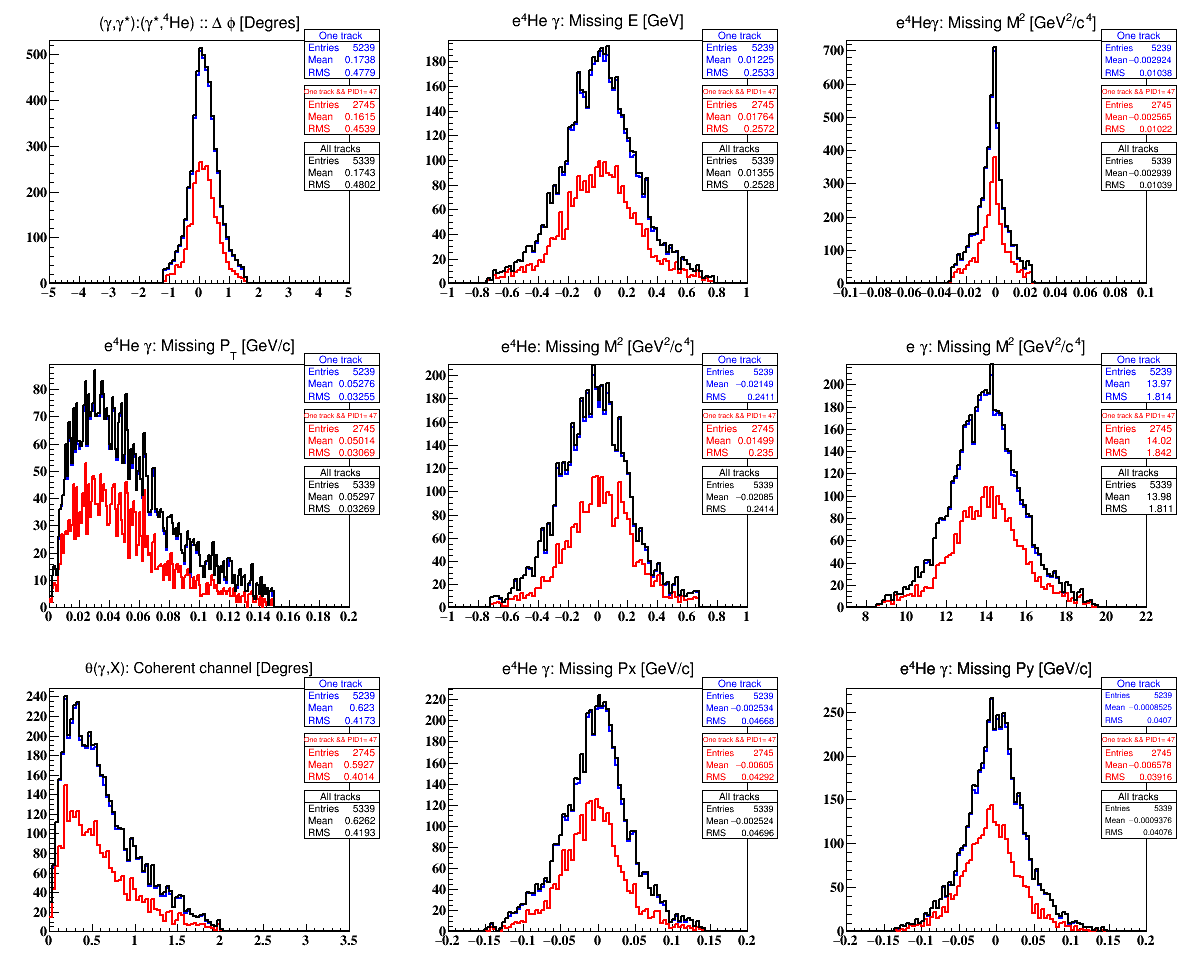
\includegraphics[height=14.2cm]{fig_dvcs/all_coh_pid.png}
      \caption{Distributions of the exclusive variable for the identified DVCS 
      events with only one track in the RTPC (blue), one track and PID1 is 
      equal to 47 (red), and processing all the tracks in each event with the 
      exclusivity variables (black).}
      \label{fig:dedx_check}
\end{figure}


In this analysis We claim that kinematic exclusivity cuts are sufficient to
cleanly select coherent $^4$He DVCS events without the need for $\frac{dE}{dx}$
cuts. We performed few checks regarding applying a PID cut, where the full data
was analyzed in the following three sets:
\begin{itemize}
\item Processing all the reconstructed tracks in each event with the exclusivity
cuts.
\item Processing events with only one good track in the RTPC being
reconstructed.
\item Processing events with only one track that passes a dedx cut.
\end{itemize}

The results are shown in figure \ref{fig:dedx_check} in terms of the
exclusive variables for the identified coherent DVCS events. One can see that
applying a PID cut would only change the statistics and not the width of
distributions. On the other hand, figure \ref{fig:coh_alu_PID} shows a 
comparison between the reconstructed beam-spin asymmetries with and without 
applying a PID cut. The two sets of asymmetries are compatible within the given 
statistical error bars. From these two observations, we deduce that a PID cut 
on the Helium would not reduce any background contribution.
   \begin{figure}[tbp]
         \centering
         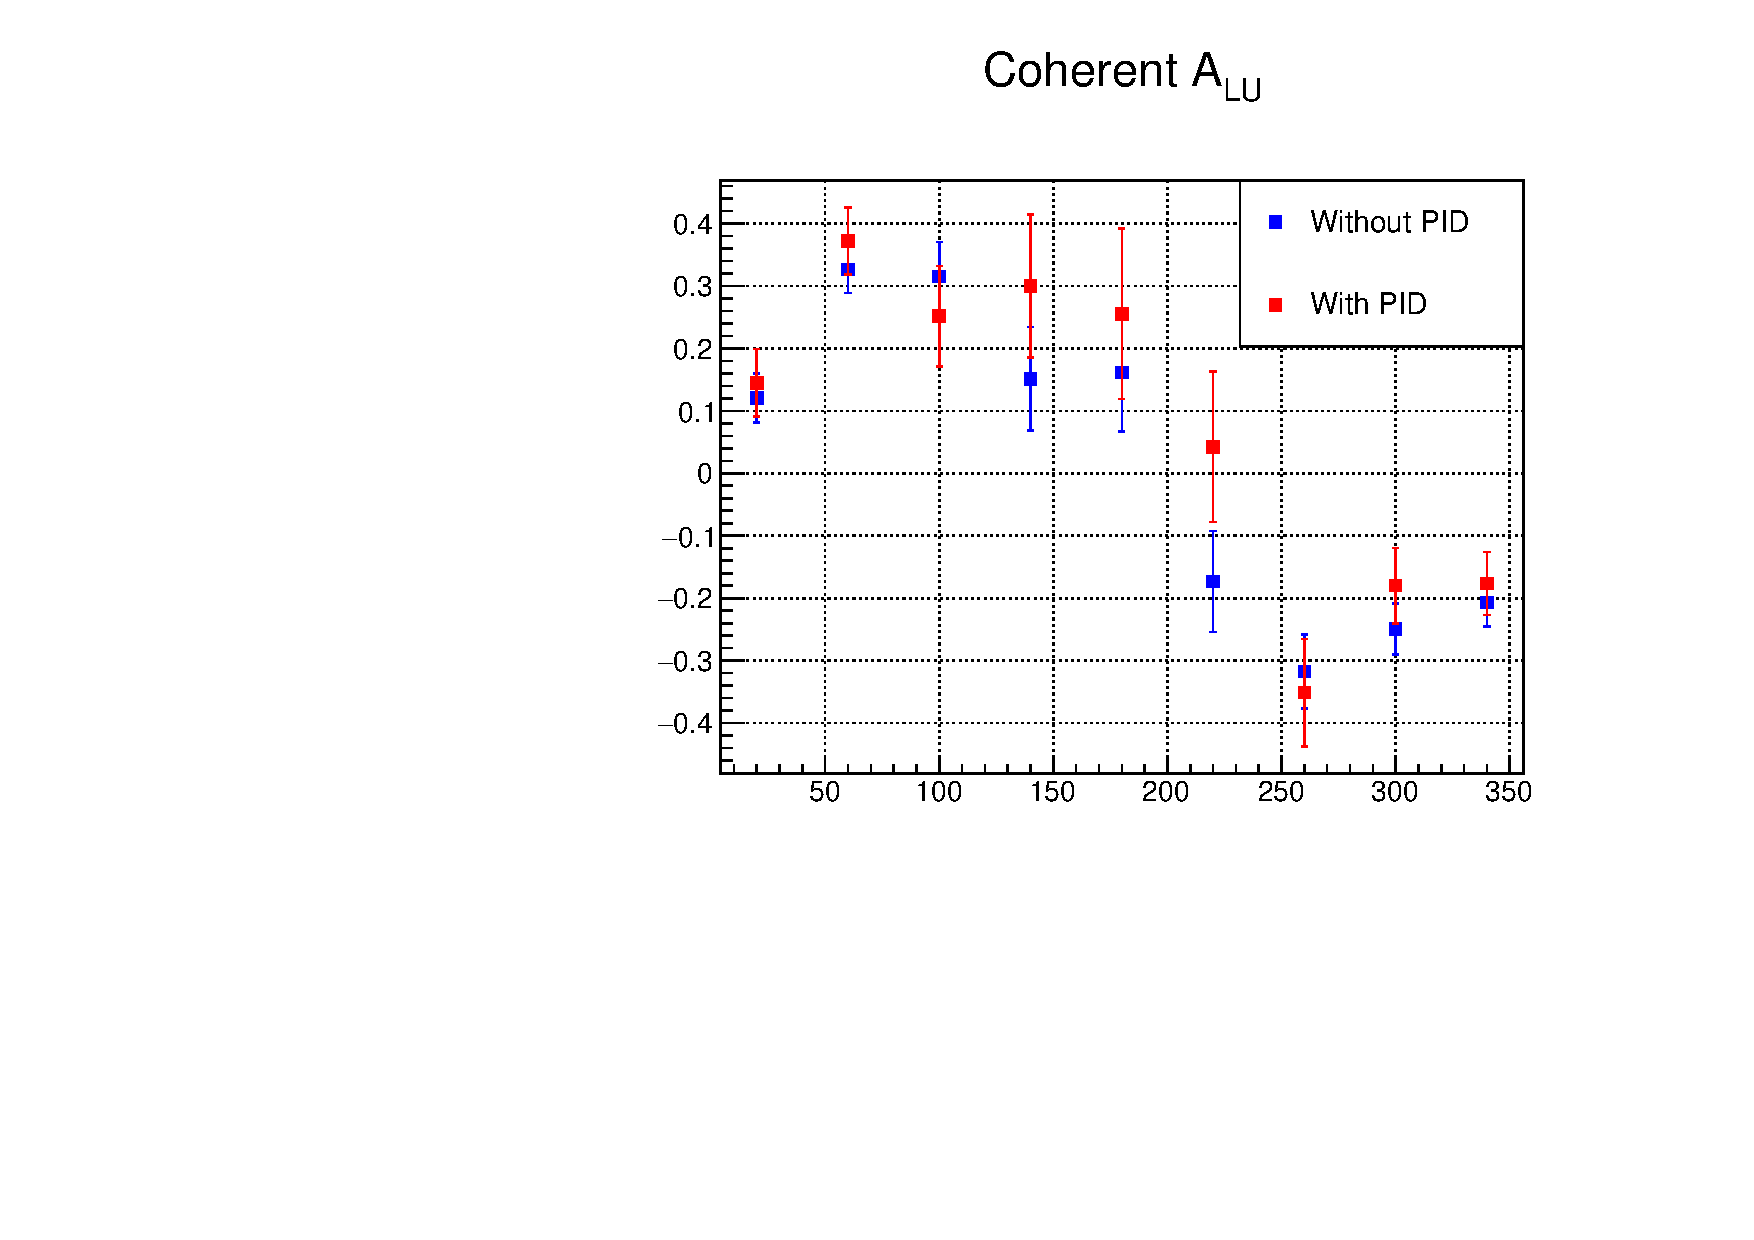
\includegraphics[height=8.2cm]{fig_dvcs/Coh_ALU_W_out_PID.pdf}
         \caption{The integrated coherent beam-spin asymmetries as a function 
         of $\phi$ with (red) and without (blue) applying a PID cut on Helium 
      tracks.}
         \label{fig:coh_alu_PID}
      \end{figure}



\subsubsection{Left/Right modules of the RTPC}
The two modules of the RTPC have shown different yields in terms of the 
identified good track, see Section 3.1.4. This different yields should not 
affect the DVCS distributions neither the reconstructed beam-spin asymmetries.  
In this section, we carry out the analysis for the coherent channel based on 
the Left/Right modules of the RTPC to ensure that the reconstructed asymmetries 
for the two modules of the RTPC are compatible. Figure 
\ref{fig:sides_rtpc_exclusivity} shows the RTPC module dependent exclusive 
distributions for the identified coherent DVCS events. Figure 
\ref{fig:coherent_alu_sides} shows the integrated coherent beam-spin 
asymmetries for the two modules separately, and for the two half together. To 
conclude, the two modules of the RTPC show a very similar performances in terms 
of the DVCS exclusive distributions and the module-dependent asymmetries are 
compatible.

\begin{figure}[tbp]
      \centering
      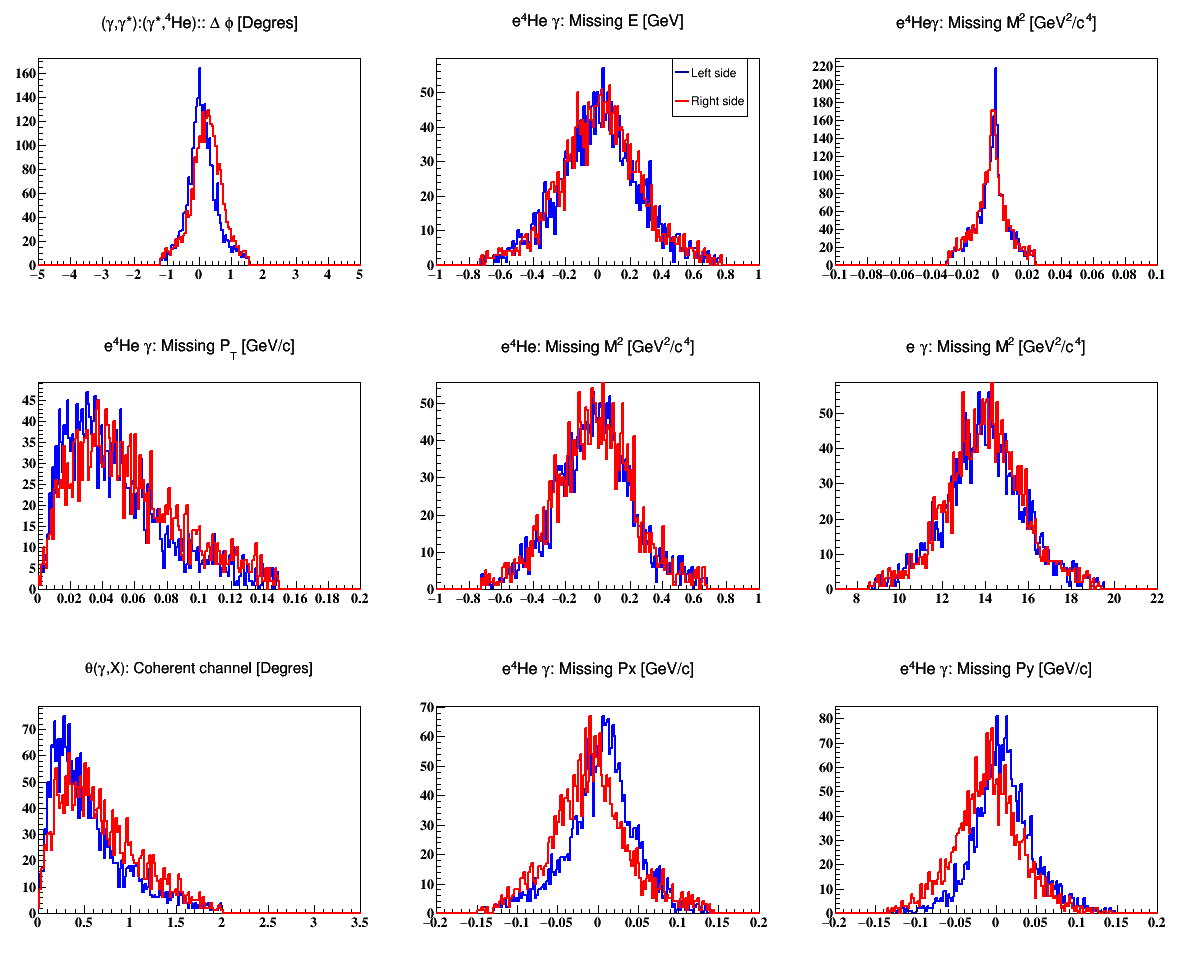
\includegraphics[height=14.2cm]{fig_dvcs/all_coh_exc_cuts_final_sides.png}
      \caption{The distributions of the exclusive variables for the identified
      coherent DVCS events in the individual modules of the RTPC, Left module 
   in blue and Right module in red.}                             
   \label{fig:sides_rtpc_exclusivity}
   \end{figure}

   \begin{figure}[tbp]
      \centering
      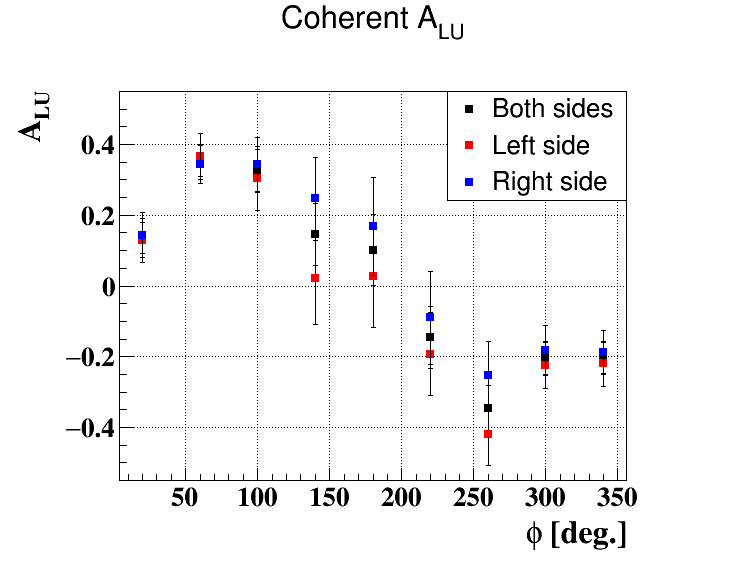
\includegraphics[height=7.0cm]{fig_dvcs/BSA_Coherent_sides.png}
      \caption{The reconstructed integrated-over-full-data beam-spin 
      asymmetries as a function of the hadronic angle $\phi$ in the two modules 
   of the RTPC separately, and the integrated signal over the whole RTPC.}
      \label{fig:coherent_alu_sides}
       \end{figure}




\subsection{Comparison with simulation}
Coherent DVCS events were simulated according to the procedures described 
in section \ref{Event_generator}. Then, events are selected following the same 
identification criteria as for the experimental data. Finally, We apply similar 
exclusivity cuts as presented for the experimental coherent DVCS events. That 
is each exclusive distribution is fitted by a Gaussian and a 3$\sigma$ cut is 
applied. So the cut are not identical, but obtained with the same method. This 
is done to avoid issues on variables where the peak is not in the exact same 
place in simulation and in data.

Figure \ref{fig:coh_comparison_with_simulation_1} shows the comparison between 
the experimental and the simulated DVCS events as a function of the kinematic 
variables: $Q^{2}$, $x_{B}$, $-t$, and $\phi$. Figure 
\ref{fig:coh_comparison_with_simulation_2} shows the comparison as a function 
of the quantities used for the exclusivity cuts. The distributions in the 
latter two figures show a satisfying match between the experimental and the 
simulated data.
\begin{figure}[h!]
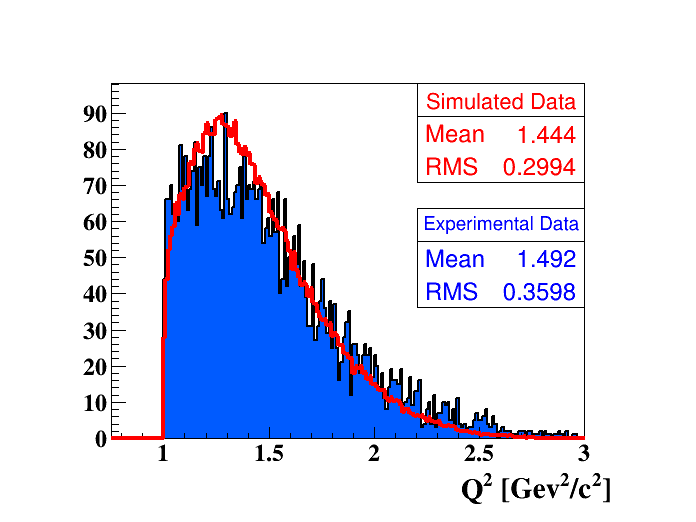
\includegraphics[scale=0.31]{fig_dvcs/comp/Q2_Coh.png}
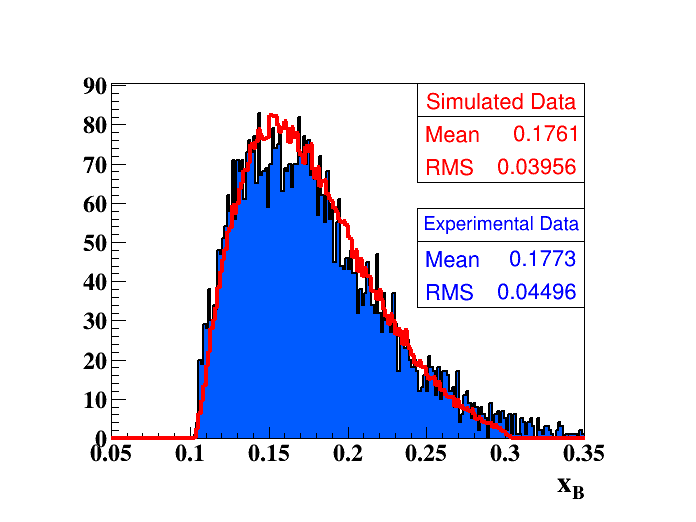
\includegraphics[scale=0.31]{fig_dvcs/comp/xB_Coh.png}
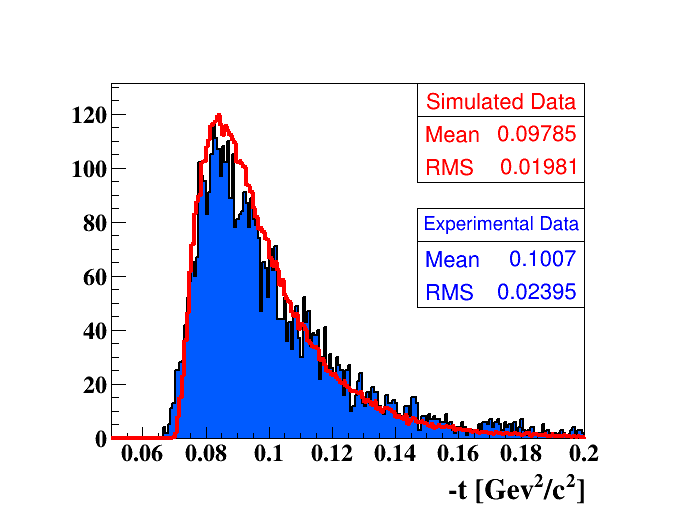
\includegraphics[scale=0.31]{fig_dvcs/comp/t_Coh.png}
\hspace{+0.5in}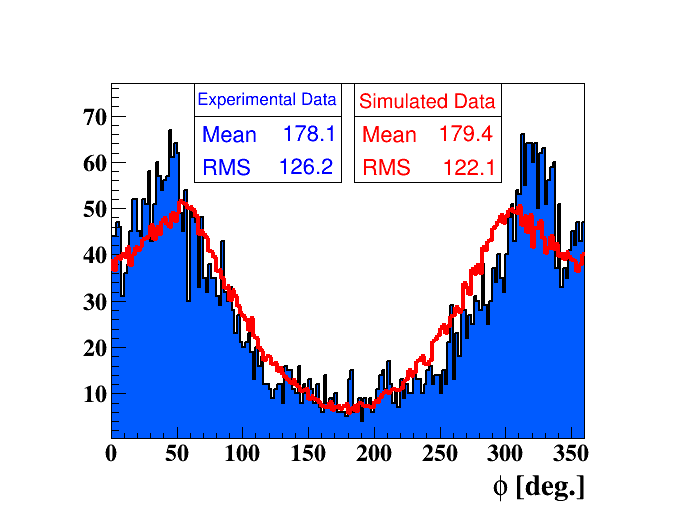
\includegraphics[scale=0.31]{fig_dvcs/comp/phi_h_Coh.png}
\caption{Comparison between the simulated $e^{4}He\gamma$ DVCS events (in red 
lines) and the experimental DVCS events (in shaded blue) as a function of the 
kinematic variables: $Q^{2}$, $x_{B}$, $-t$, and $\phi$. }
\label{fig:coh_comparison_with_simulation_1}
\end{figure}

\begin{figure}[h!]
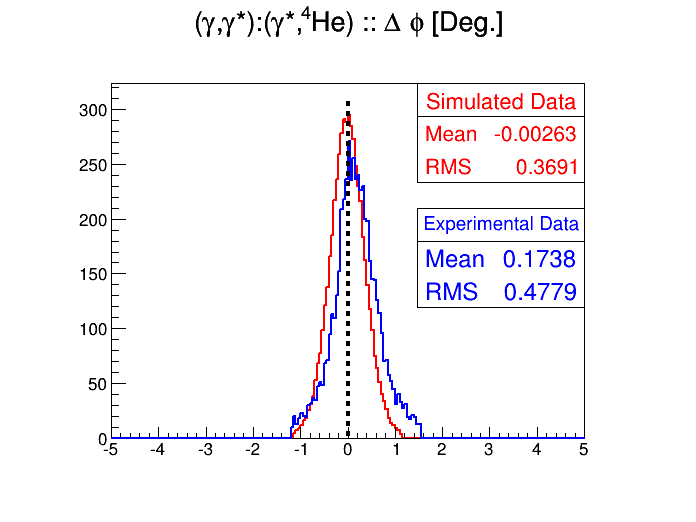
\includegraphics[scale=0.36]{fig_dvcs/comp/Coh_delta_phi.png}
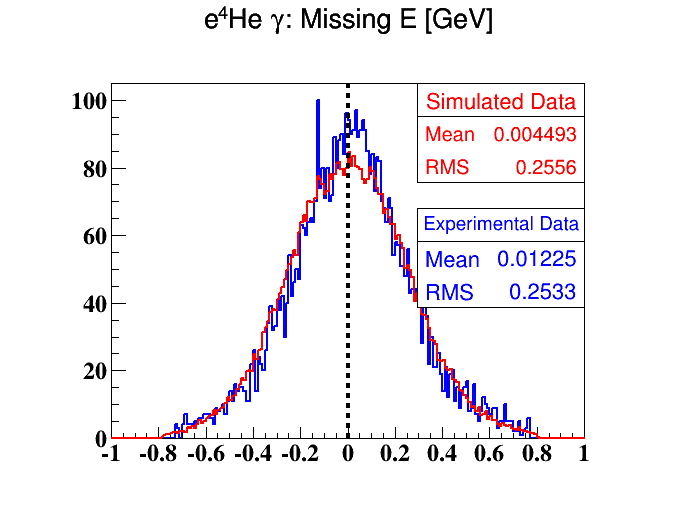
\includegraphics[scale=0.36]{fig_dvcs/comp/Coh_e4Hegamma_E_Mis.png}
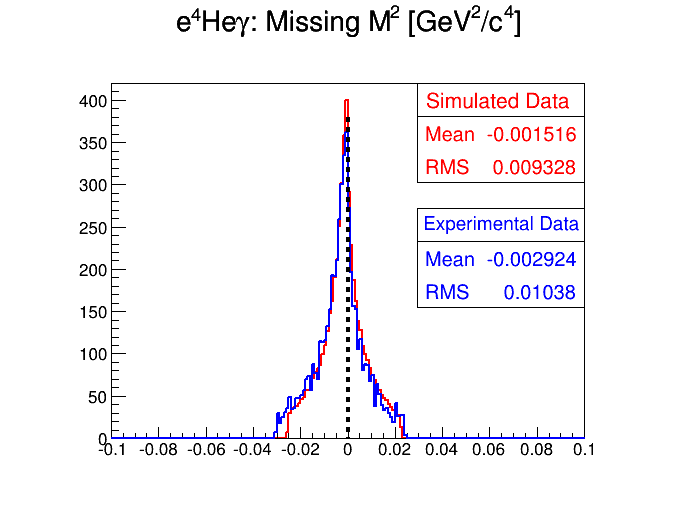
\includegraphics[scale=0.36]{fig_dvcs/comp/Coh_e4Hegamma_M2_Mis.png}
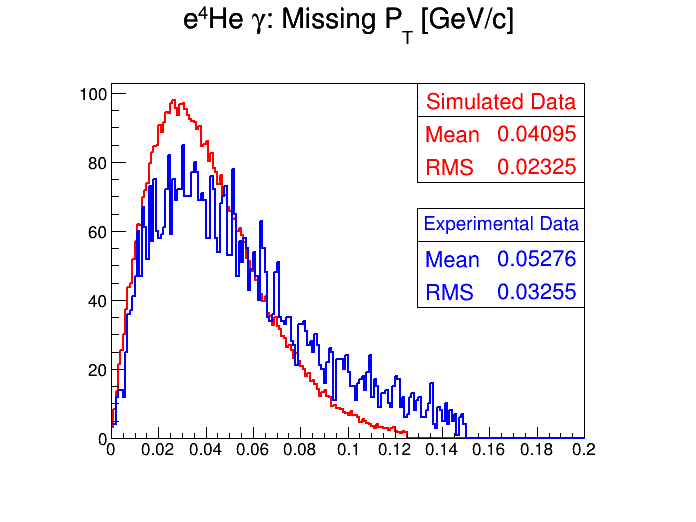
\includegraphics[scale=0.36]{fig_dvcs/comp/Coh_e4Hegamma_PT_Mis.png}
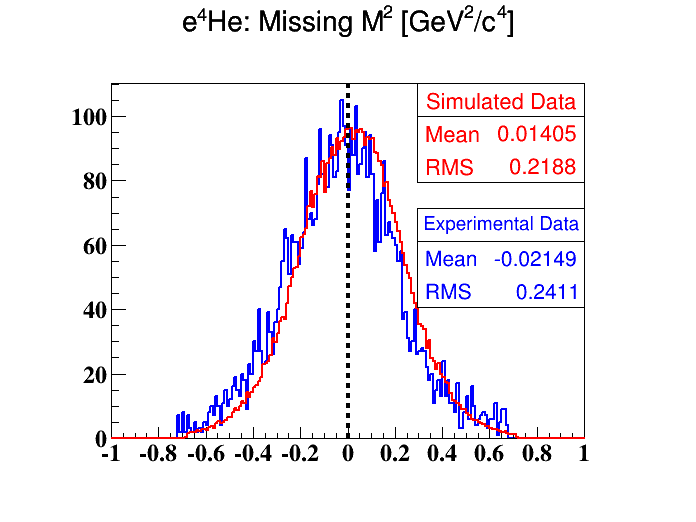
\includegraphics[scale=0.36]{fig_dvcs/comp/Coh_e4He_M2_Mis.png}
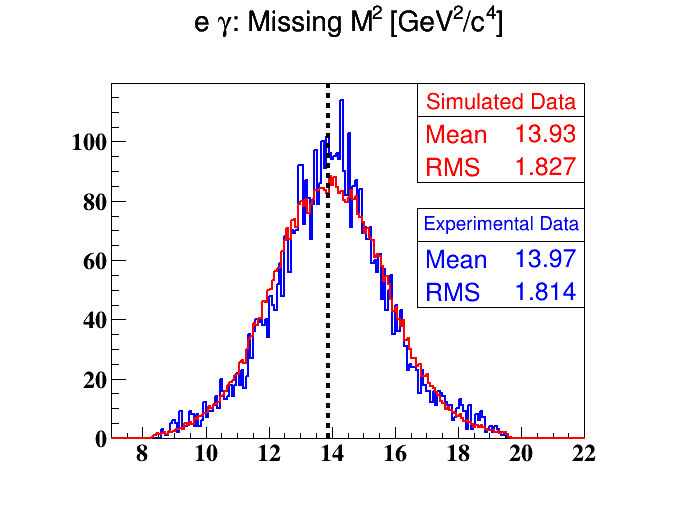
\includegraphics[scale=0.36]{fig_dvcs/comp/Coh_egamma_M2_Mis.png}
\caption{Comparison between simulated and experimental $e^{4}He\gamma$ DVCS events. The distributions from left to right and from top to bottom are: Co-planarity cut, missing energy, missing mass squared and missing transverse momentum in the configuration of detecting all the three final-state particles, missing mass squared in the $e^{4}HeX$ and $e\gamma X$ configurations respectively. The vertical black lines indicate the theoretically expected value for each quantity.} 
\label{fig:coh_comparison_with_simulation_2}
\end{figure}

  

~\newpage
~\newpage

\section{Incoherent channel}
In this channel, the DVCS process happens on a bound proton. Thus, the 
final state has a recoil proton instead of the helium nucleus. Therefore, 
events with one good electron, one recoil proton, and at least one real photon 
are the good candidates here. For the rest, we follow the same steps that were 
introduced for the coherent DVCS selection.

\subsection{Good run list}
The events rate stability is verified by looking at the rate of the 
detected number of protons to the detected electrons (<p/e>). Like for the 
coherent channel, the same technique for the determination of the good run list 
is followed herein. The results are presented in figure 
\ref{fig:prot_over_e_Run_sec.png}.  \begin{figure}[h!]
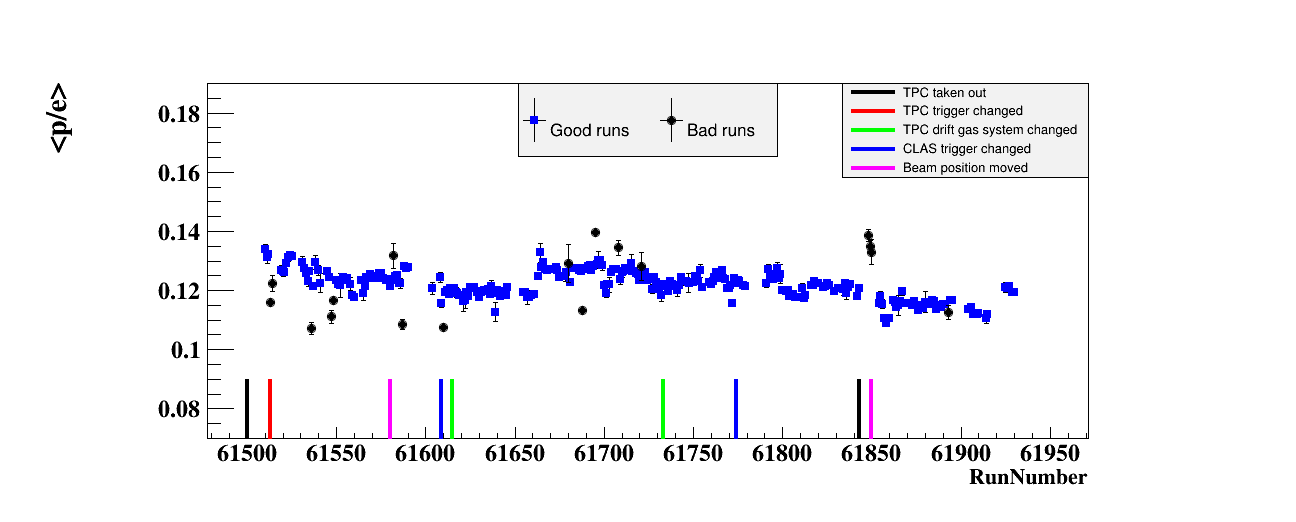
\includegraphics[scale=0.4]{fig_dvcs/prot_over_e_Run.png}
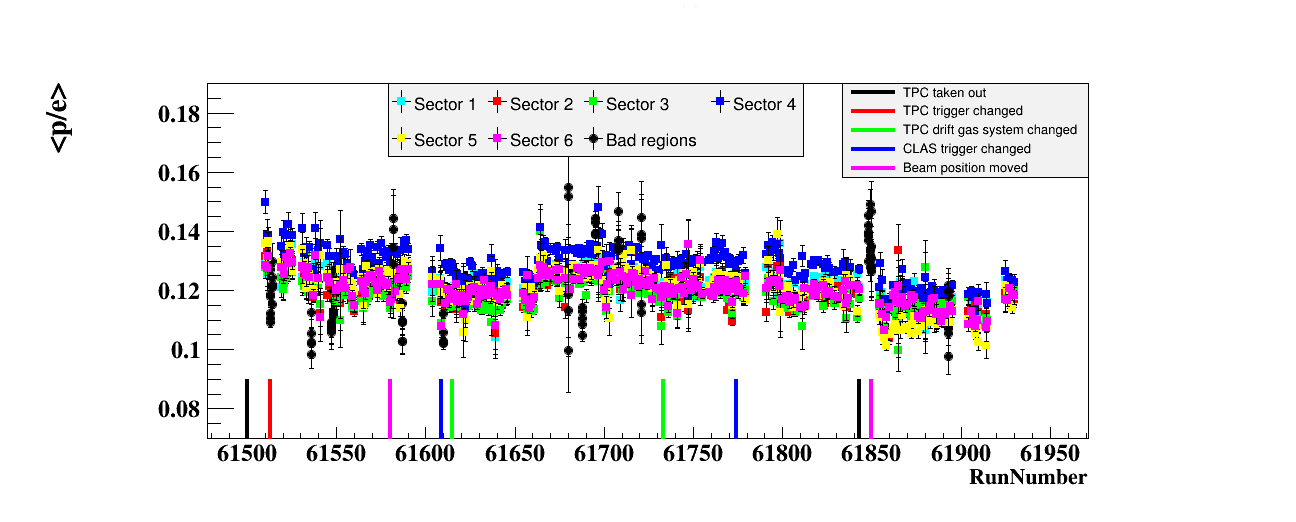
\includegraphics[scale=0.4]{fig_dvcs/prot_over_e_Run_sec.png}
\caption{On the top: the integrated <$p/e$> ratio as a function of run number.  
   The blue points refer to the good runs, while the black points are the 
rejected ones. On the bottom: the same ratio for each run, is shown for each 
sector of CLAS. The colored points indicate the six sectors, while the black 
points are the sectors of the rejected runs. } 
\label{fig:prot_over_e_Run_sec.png}
\end{figure}


\subsection{Proton DVCS event selection}
To certify that an event is a proton DVCS one, we require the same DVCS 
kinematic cuts as those presented for the coherent DVCS selection. Then, the 
exclusivity of the DVCS reaction is ensured by applying an equivalent set of 
exclusivity with taking a proton at rest as the target, instead of $^4He$.  
Figure \ref{fig:incoh_exclusivty_cuts} summarizes these exclusivity cuts.

%\paragraph{$\blacklozenge$ DVCS characteristics}
%\begin{itemize}
%\item The invariant mass of the system of the virtual photon and the target proton is greater than $2~GeV/c{^2}$ in order to avoid the excitation of the proton to baryon states and be above the nucleon resonances.
%\item $Q2 > 1 GeV^{2}$: To ensure that we have hard interaction and the applicability of the handbag diagram factorization for the DVCS.
%\item High energetic final state real photon ($E_{\gamma}> 2 GeV$)
%\item $ -t > t_{min}$: The transferred momentum squared to the proton has to be greater than a minimum value defined by the kinematics of the beam and the scattered electron as:
%\begin{equation}
%t_{min} = \frac{- Q^{2}*2(1- x_{B})(1 + \epsilon ^{2} - \sqrt{1 + \epsilon ^{2}})}{4 x_{B}(1-x_{B})+ \epsilon ^{2};}\\
%\end{equation}
%Where $\epsilon ^{2} = \frac{4M^{2}_{p}x^{2}_{B}}{Q^{2}}$.
%\end{itemize}

%\paragraph{$\blacklozenge$ Exclusivity cuts}~
%~~~~The exclusivity of the proton DVCS events is ensured by applying the following set of cuts:
%\begin{itemize}
%\item The coplanarity cut ($\Delta \phi$) between the recoil proton and the final state real photon. 
%\item Missing energy, mass and transverse momentum ($p_{T} = \sqrt{p^{2}_{x} + p^{2}_{y}}$) cuts in the final state configuration $ep\gamma X$.
%\item Missing mass cuts in the final state configurations $epX$ and $e\gamma X$.
%\item Cone angle cut between the measured real photon and the missed particle in the %configuration $epX$.
%\end{itemize}
\begin{figure}[h!]
\centering
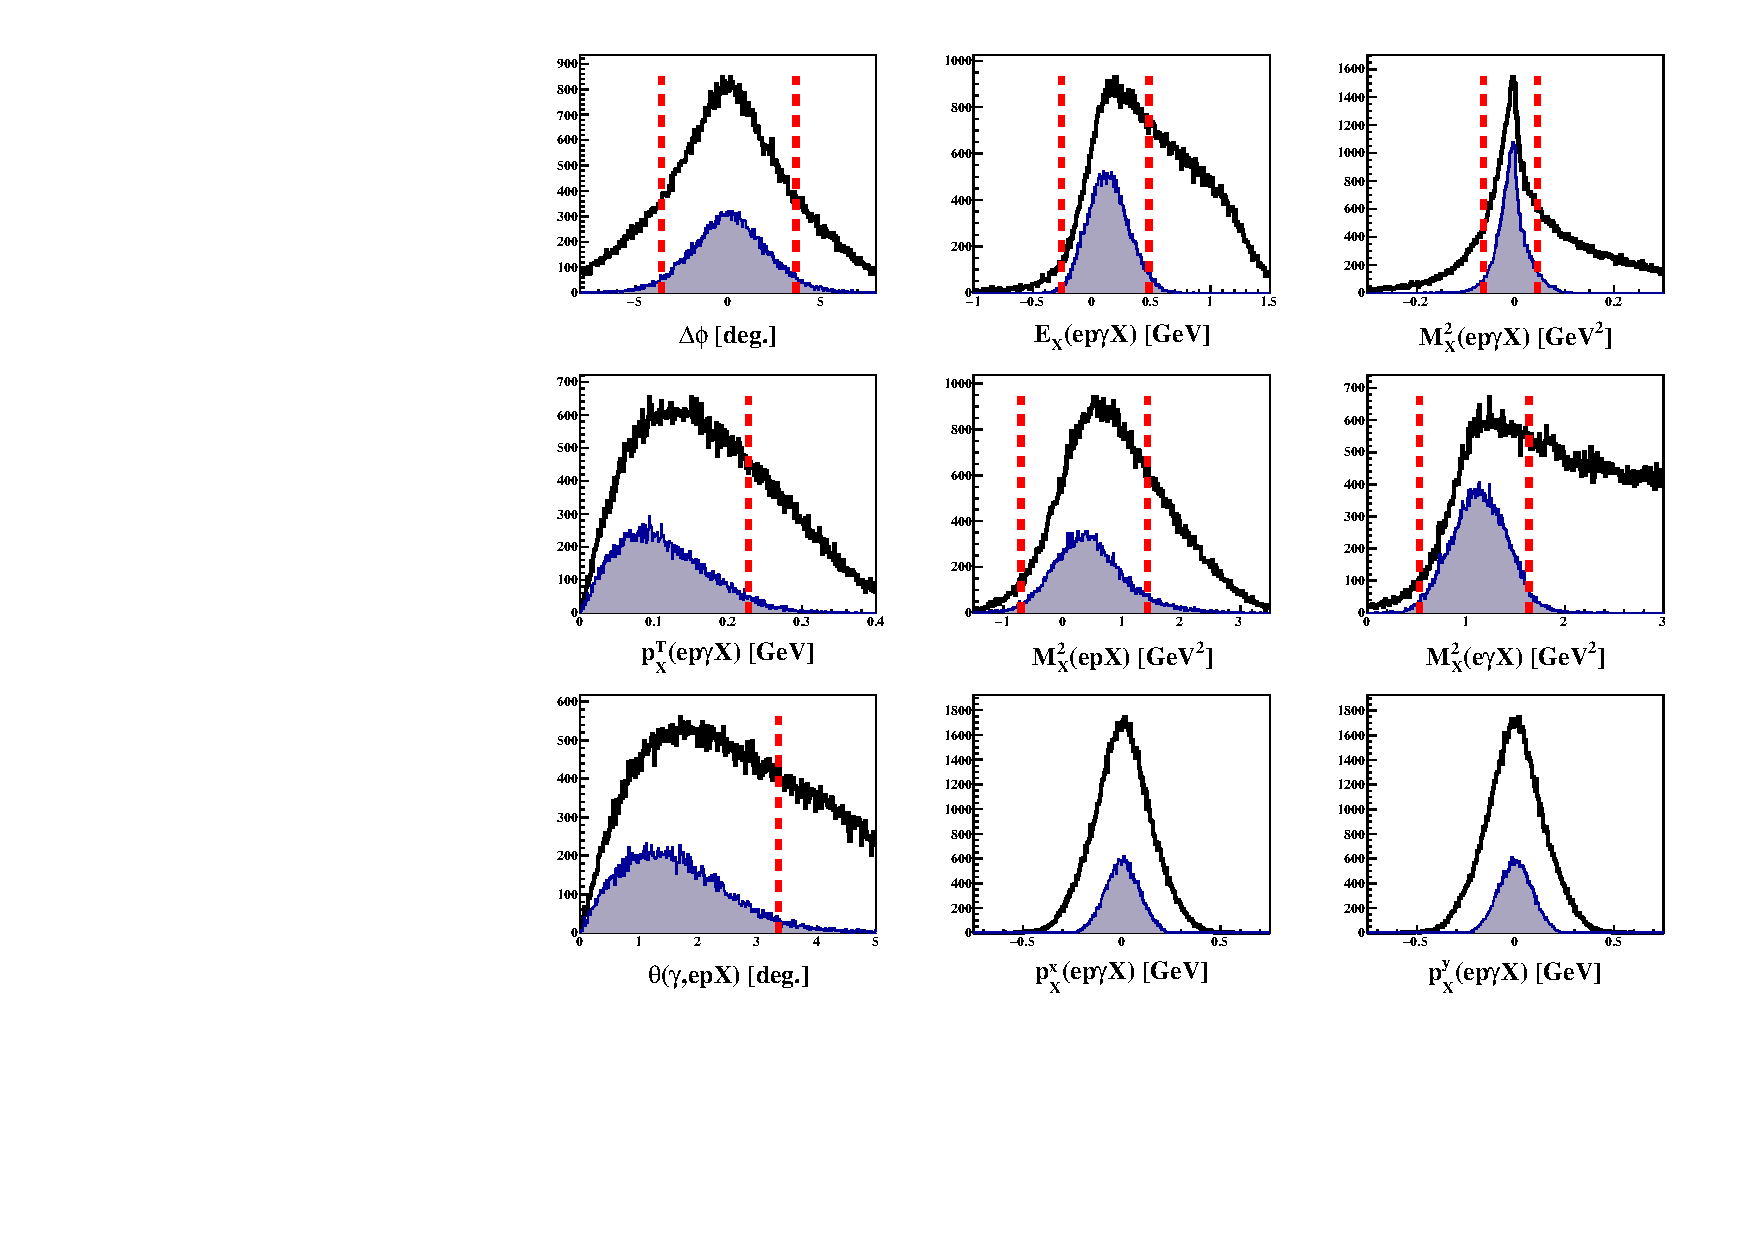
\includegraphics[scale=0.9]{fig_Dec2016/all_incoh_exc_cuts.pdf}
\caption{The incoherent DVCS exclusivity cuts. The black distributions 
   represent all the events with one good electron, one good proton, and at 
   least one photon in the IC. The shaded brown distributions show the 
   incoherent DVCS events which passed all the exclusivity cuts except the one 
   on the quantity drawn. The distributions from left to right and from top to 
   bottom are: the proton-photon coplanarity, the missing energy, missing mass 
   squared, missing transverse momentum from $ep\gamma X$, the missing mass 
   squared $epX$ and the missing mass squared $e\gamma X$, the angle between 
   the missing particle in $epX$ and the measured photon, the missing $P_{x}$ 
   and $P_{y}$ in $ep\gamma X$. The vertical red lines represent 3$\sigma$ 
   cuts. The mean and sigma values of each shaded distribution are listed in 
table \ref{Table:incoh_exclusivity_cuts}.} \label{fig:incoh_exclusivty_cuts}
\end{figure}

\subsection{Comparison with simulation}
The three particles of the simulated $ep\gamma$ DVCS events are selected 
applying the previously described identification requirements. The events with 
three identified particles (e, p, $\gamma$) are required to pass a set of 
exclusivity cuts such as the ones of the experimental incoherent DVCS events.  
In this section, a comparison between the experimental and the simulated data 
is carried out.

Figure \ref{fig:incoh_coparison_with_simulation_1} shows the comparison between 
the simulated (red lines) and the experimental (shaded blue) incoherent DVCS 
events as a function of the four kinematic variables: $Q^{2}$, $x_{B}$, $-t$, 
and $\phi$. Figure \ref{fig:incoh_comparison_with_simulation_exclusive_2} shows 
the comparison as a function of the variables used to select exclusive DVCS 
events.
\begin{figure}[h!]
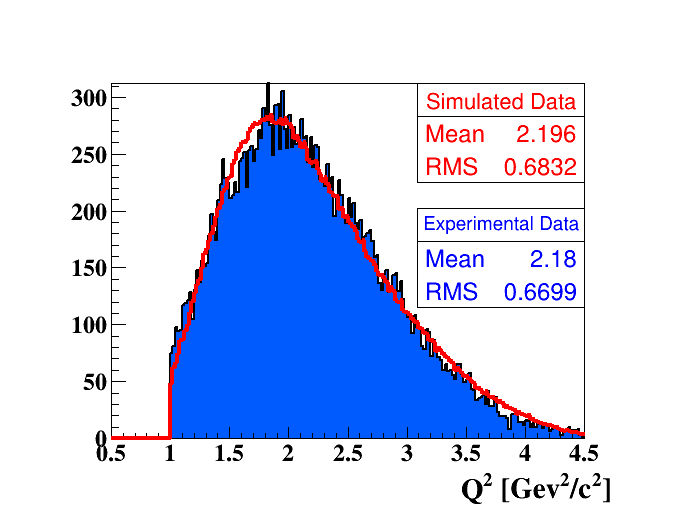
\includegraphics[scale=0.35]{fig_dvcs/comp/Q2_InCoh.png}
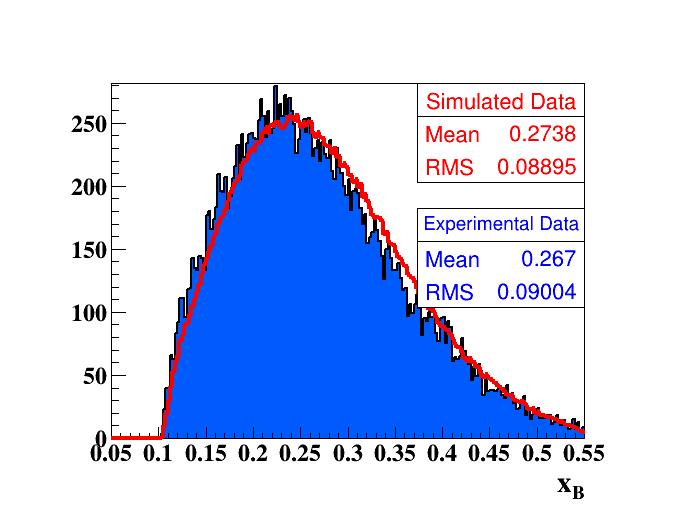
\includegraphics[scale=0.35]{fig_dvcs/comp/xB_InCoh.png}
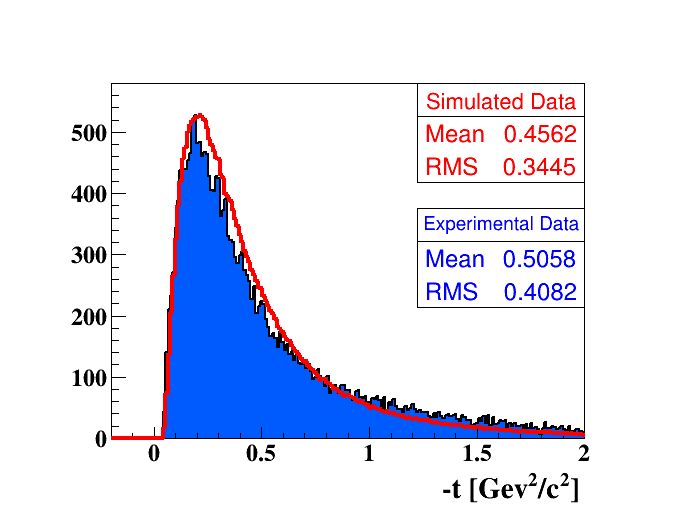
\includegraphics[scale=0.35]{fig_dvcs/comp/t_InCoh.png}
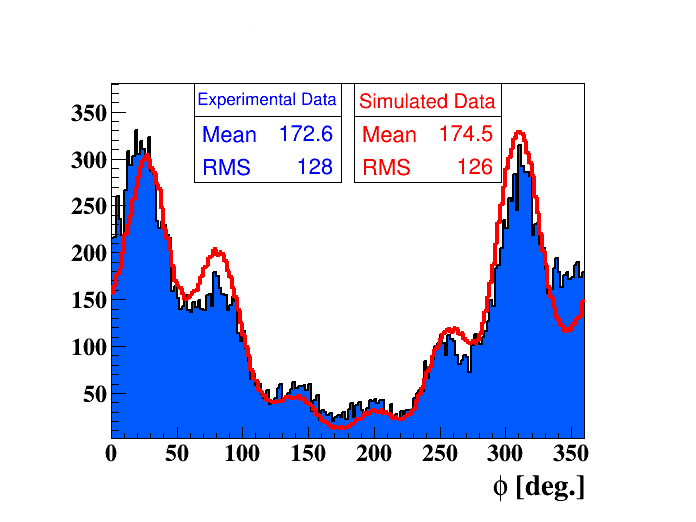
\includegraphics[scale=0.35]{fig_dvcs/comp/phi_h_InCoh.png}
\caption{Comparison between the Monte-Carlo simulated $ep\gamma$ DVCS events 
(red lines) and the experimental ones (blue shaded distributions) in terms of 
the kinematics: $Q^{2}$, $x_{B}$, $-t$, and $\phi$, respectively from left to 
right and from top to bottom.}
\label{fig:incoh_coparison_with_simulation_1}
\end{figure}


\begin{figure}[h!]
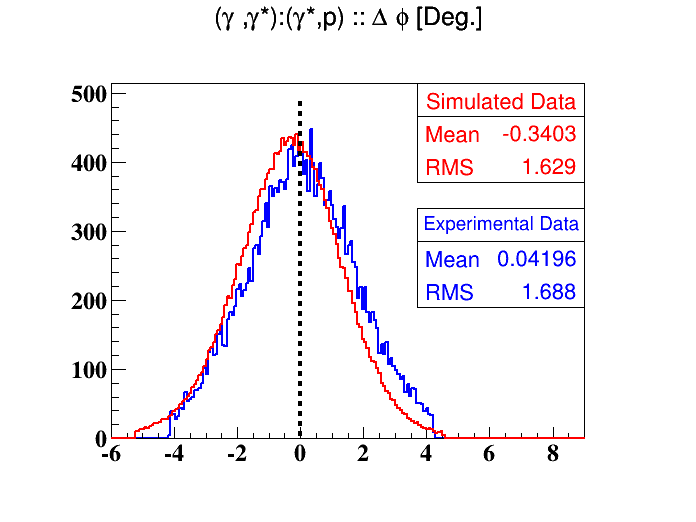
\includegraphics[scale=0.35]{fig_dvcs/comp/InCoh_delta_phi_InCoh.png}
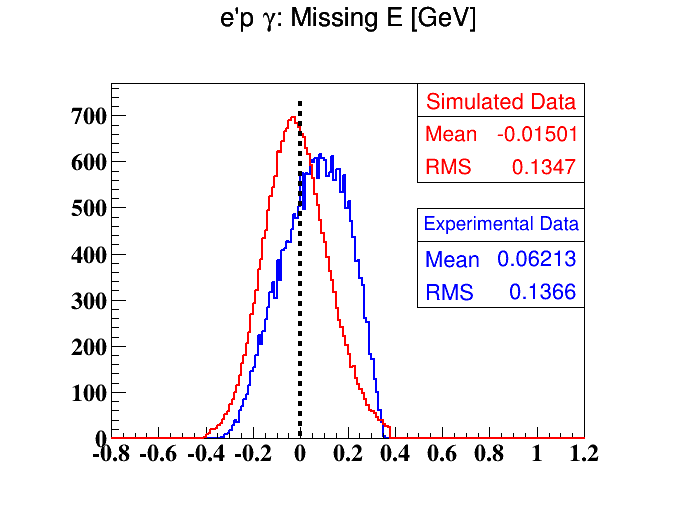
\includegraphics[scale=0.35]{fig_dvcs/comp/InCoh_epgamma_E_Mis.png}
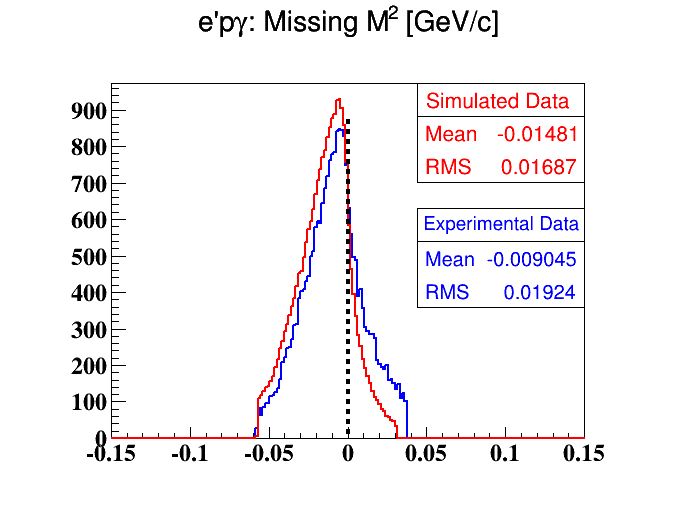
\includegraphics[scale=0.35]{fig_dvcs/comp/InCoh_epgamma_M2_Mis.png}
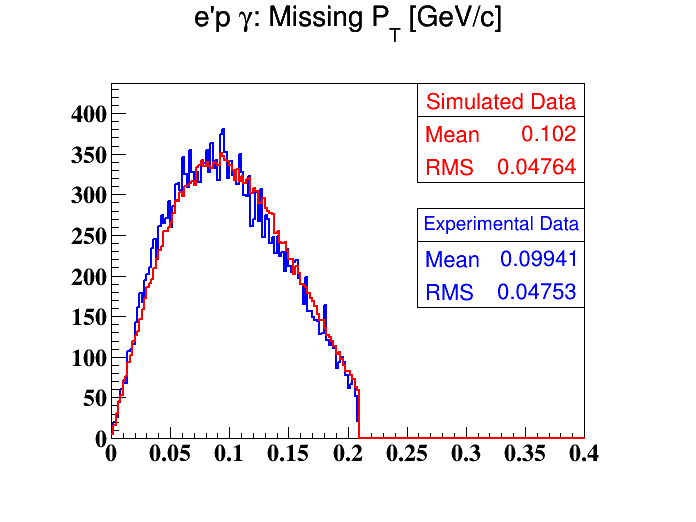
\includegraphics[scale=0.35]{fig_dvcs/comp/InCoh_epgamma_PT_Mis.png}
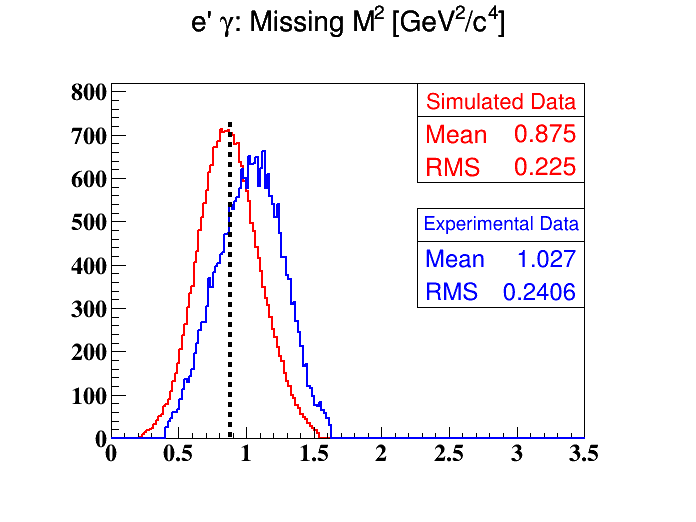
\includegraphics[scale=0.35]{fig_dvcs/comp/InCoh_egamma_M2_Mis_InCoh.png}
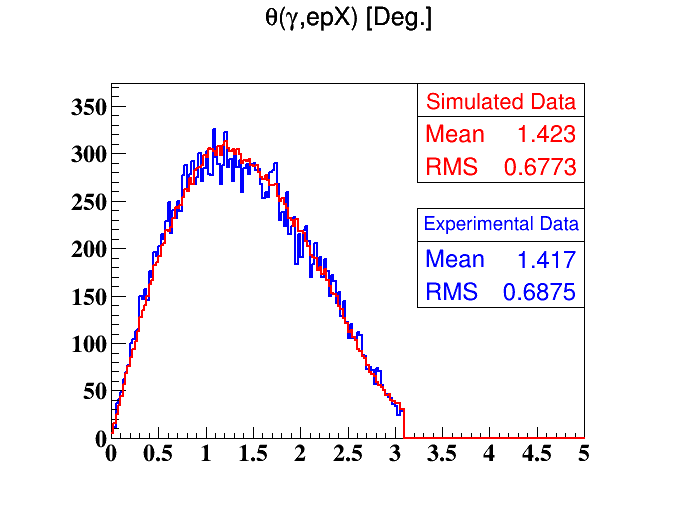
\includegraphics[scale=0.35]{fig_dvcs/comp/InCoh_Theta_gammaX_InCoh.png}
\caption{Comparison between simulated and experimental $ep\gamma$ DVCS events 
in terms of the variables used for exclusivity cuts. The vertical black lines 
indicate the theoretically expected values for each exclusive quantity.} 
\label{fig:incoh_comparison_with_simulation_exclusive_2}
\end{figure}

~\newpage
~\newpage
\section{Kinematic coverages}
The one-dimensional distributions of explored kinematical regions can be 
seen in figure \ref{fig:coh_comparison_with_simulation_1} for the coherent, and 
in figure \ref{fig:incoh_coparison_with_simulation_1} for the incoherent DVCS 
channels. In figure \ref{fig:kinematic_coverage}, we show two-dimensional 
distributions of these variables to display the correlations between them. 
%\begin {table}[!h]
%\begin{center}
%\begin{tabular}{|l|l|l|l|}
%\hline
%DVCS channel &  $Q^{2}$~$[GeV^{2}/c^{2}]$  & $~~~~~~x_{B}$  & -t ~$[GeV^{2}/c^{2}]$\\
%\hline
%Helium-4 & [1.0, 3.0] & [0.1, 0.3] & [0.06, 0.2] \\
%\hline
%proton & [1.0, 4.5] & [0.1, 0.55] & [0.03, 2.5] \\
%\hline
%\end{tabular}
%\caption{ The coherent and the incoherent explored kinematic regions.}
%\label{Table:kinematic_ranges}
%\end{center}
%\end{table}

\begin{figure}[h!]
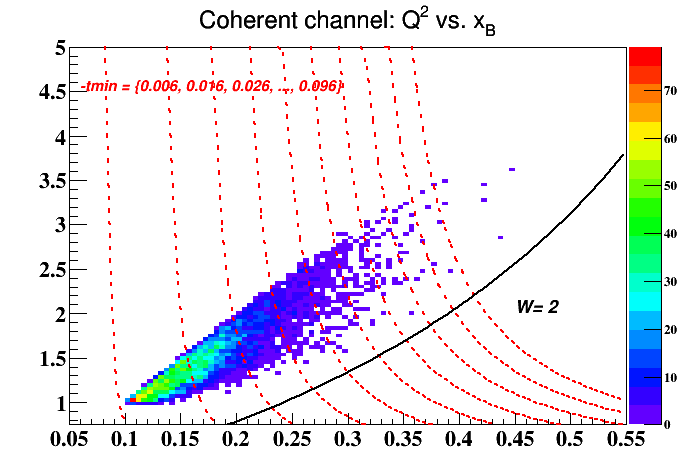
\includegraphics[scale=0.35]{fig_dvcs/coh_Q2_xB.png}
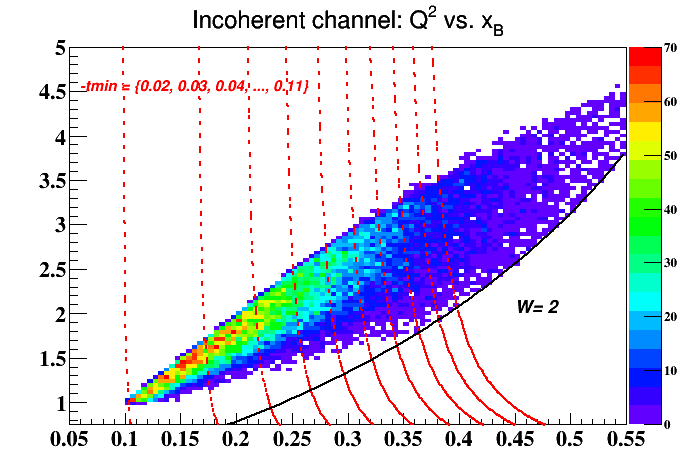
\includegraphics[scale=0.35]{fig_dvcs/incoh_Q2_xB.png}
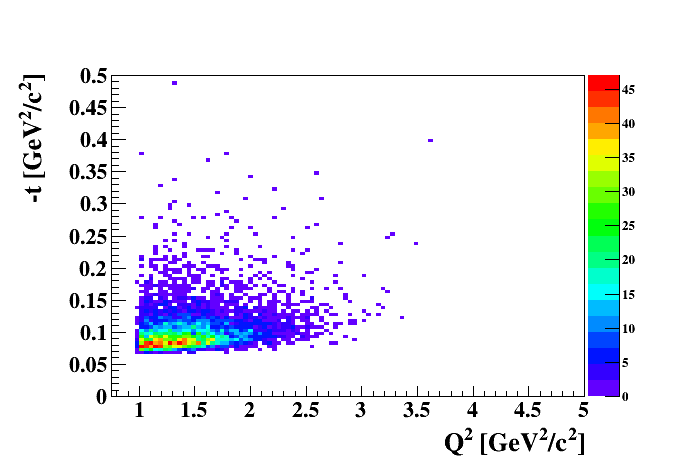
\includegraphics[scale=0.35]{fig_dvcs/new_t_Q2_Coh.png}
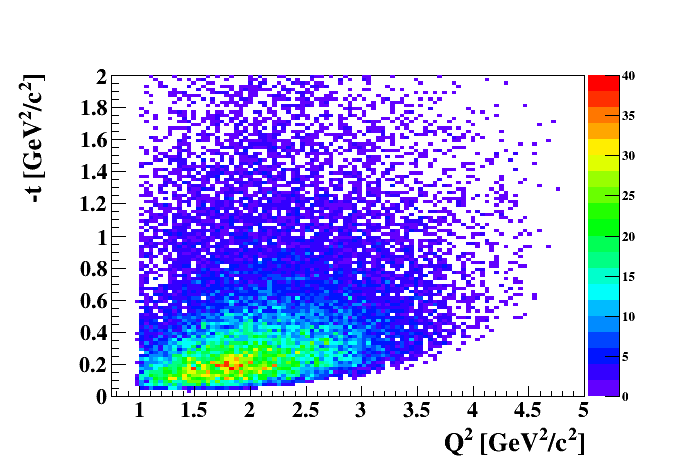
\includegraphics[scale=0.35]{fig_dvcs/new_t_Q2_InCoh.png}
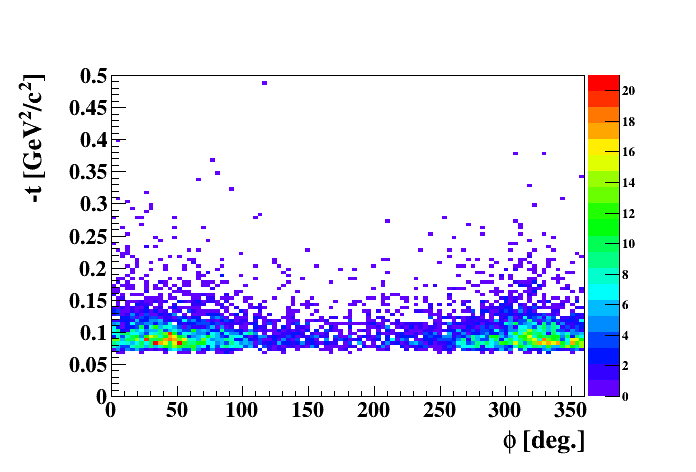
\includegraphics[scale=0.35]{fig_dvcs/new_phi_t_Coh.png}
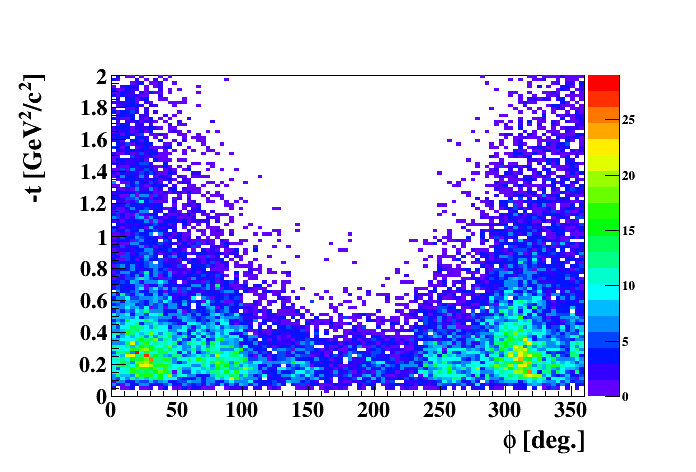
\includegraphics[scale=0.35]{fig_dvcs/new_phi_t_InCoh.png}
\caption{The distributions of the identified coherent DVCS are on the left 
   panel, while on the right are the incoherent ones. On the top panel: $Q^2$ 
as a function of $x_B$ with W and fixed $-t_{min}$ value cuts in $Q^{2}-x_{B}$ 
plane. On the middle panel: $-t$ as a function of $Q^2$.  On the bottom panel: 
$-t$ as a function of $\phi$.} \label{fig:kinematic_coverage}
\end{figure}

\section{Data binning}
The DVCS cross section and $A_{LU}$, equations \ref{BSA_equation} to 
\ref{eq:A_LU-coh}, depend on the four kinematic variables: $Q^{2}$, $x_{B}$, 
$t$, and $\phi$. The number of identified coherent (incoherent) DVCS events is 
about 5000 (30k). Due to our limited statistics only, a two-dimensional binning 
is carried out in this analysis.  The strongest dependence of $A_{LU}$ is on 
the azimuthal angle between the leptonic and the hadronic planes ($\phi$).  
Thus, we construct the two-dimensional bins as follows: the coherent 
(incoherent) measured ranges of $Q^{2}$, $x_{B}$ and $-t$ are binned 
statistically into three (four) bins.  Then, the identified DVCS events in each 
$Q^{2}$, $x_{B}$ and $-t$ bin, are binned into nine bins in $\phi$.  Therefore, 
we are left with $Q^2$-$\phi$ bins integrated over the full ranges of $x_{B}$ 
and $-t$, $x_{B}$-$\phi$ bins integrated over $Q^2$ and $-t$, and $-t$-$\phi$ 
bins integrated over $Q^2$ and $x_{B}$. For instance, figure 
\ref{fig:coh_Q2_bins} shows the one-dimensional bins in $Q^2$ and the 
associated bins in $\phi$.

\begin{figure}[h!]
\centering
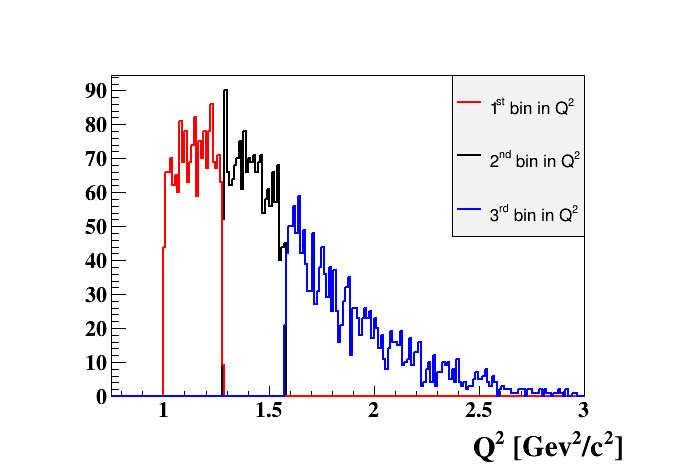
\includegraphics[scale=0.36]{fig_results/Q2_Coh_bins.png}
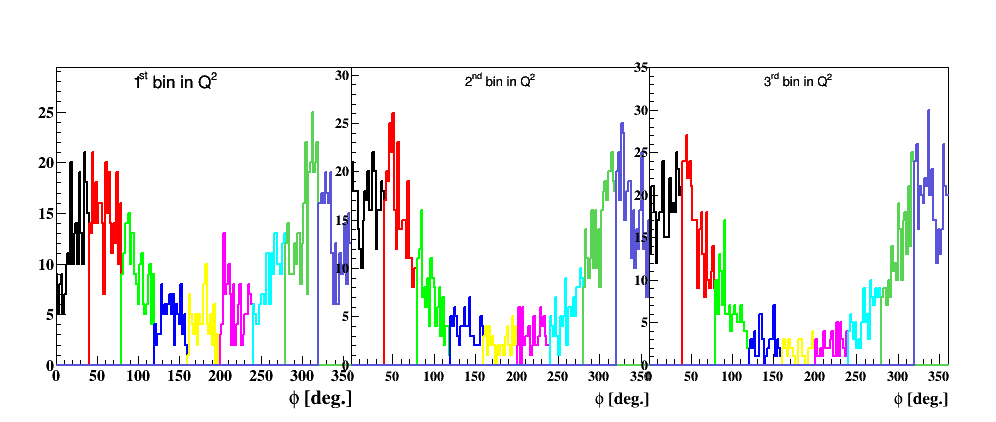
\includegraphics[scale=0.45]{fig_results/bins_Coh_Q2_Phi.png}
\caption{On the top: the $Q^2$ distribution of the collected coherent DVCS 
   events. The different colors indicate the different bins in $Q^2$ integrated 
   over the full ranges of $-t$ and $x_B$. On the bottom: the $\phi$ 
   distributions of the coherent DVCS events for the bins in $Q^2$, which are 
shown in the top plot. The different colors in each $\phi$ distribution 
represent the nine bins in $\phi$.} \label{fig:coh_Q2_bins}
\end{figure}


\section{Background subtraction}
\label{Background_subtraction}

\subsection{$\pi^0$ contaminations}
Even with all cuts applied to select the selected DVCS events, the events 
are not all DVCS events. In our kinematic region, the main contamination comes 
from the exclusive electroproduction of $\pi^{0}$ ($e ^{4}He \rightarrow e 
^{4}He \pi^{0} \rightarrow e ^{4}He \gamma \gamma $, $e p \rightarrow e p 
\pi^{0} \rightarrow e p \gamma \gamma $), in which one of the two photons of 
the $\pi^{0}$ decay passes the requirements of the DVCS. Thus, the event is 
counted as a DVCS event. These events contaminate the DVCS sample and have to 
be subtracted to obtain the true number of DVCS events. In the case of the 
coherent channel, this can be formulated as:
\begin{equation}
N^{True}_{e^{4}He\gamma} = N^{Exp.}_{e^{4}He\gamma} -  N^{Exp.}_{e^{4}He\pi^{0}(\gamma)},
\label{equ_back_1}
\end{equation}
where $N^{True}_{e^{4}He\gamma}$, $N^{Exp.}_{e^{4}He\gamma}$ and $ 
N^{Exp.}_{e^{4}He\pi^{0}(\gamma)}$ are the true number of coherent DVCS events, 
the experimentally measured number of $e^{4}He\gamma$ events and the 
contamination number, respectively. The contamination can be calculated by 
using real data and simulation. We define, for each kinematic bin and for each 
beam helicity state
\begin{equation}
N^{Exp.}_{e^{4}He\pi^{0}(\gamma)} = 
\frac{N^{Sim.}_{e^{4}He\pi^{0}(\gamma)}}{N^{Sim.}_{e^{4}He\pi^{0}(\gamma 
\gamma)}} * N^{Exp.}_{e^{4}He\pi^{0}(\gamma \gamma)},
\label{equation: background_equ}
\end{equation}
where $N^{Exp.}_{e^{4}He\pi^{0}(\gamma \gamma)}$ is the number of measured 
$e^{4}He\pi^{0}$ events, for which both photons of the $\pi^{0}$ have been 
detected. The quantity 
$\frac{N^{Sim.}_{e^{4}He\pi^{0}(\gamma)}}{N^{Sim.}_{e^{4}He\pi^{0}(\gamma 
\gamma)}} $ is the acceptance ratio for detecting a $e^{4}He\gamma$ event that 
originates from an $e^{4}He\pi^{0}$ event. It can be derived from Monte-Carlo 
simulations by generating and simulating $e^{4}He\pi^{0}$.  
$N^{Sim.}_{e^{4}He\pi^{0}(\gamma)}$ is the number of such events passing the 
DVCS requirements, while $N^{Sim.}_{e^{4}He\pi^{0}(\gamma \gamma)}$ is the 
number of simulated $e^{4}He\pi^{0}$ events passing the exclusivity cuts for 
$e^{4}He\pi^{0}$ events.

The previous formulas apply to the case of the coherent DVCS. The same 
procedures hold for the incoherent case by replacing the $^{4}He$ with the 
proton.

The selection of the exclusive $e^{4}He\pi^{0}$ and $ep\pi^{0}$ events requires 
the detection of one good electron, one good $\pi^{0}$ in the topology ICIC or 
ICEC, and one good $^{4}He$ track in the coherent case, or one good proton in 
the incoherent case. In order to ensure that this is a deep process, we apply 
the same kinematic cuts as DVCS. These cuts and the comparisons with simulation 
can be found in Appendix \ref{app:Exclusive_pi0_selection}.


Figure \ref{fig:coh_acceptance _ratios} shows the coherent acceptance ratio as 
a function of each of the four kinematic variables ($Q^{2}$, $x_{B}$, $-t$, 
$\phi_{h}$). These distributions are one-dimensional, i.e. the data are 
integrated over all kinematical ranges except for the quantity which is binned 
(along the x-axis). The results for the incoherent channel can be found in 
figure \ref{fig:incoh_acceptance _ratios}. The mean value of the acceptance 
ratio for the coherent channel is around 25$\%$, with some dependence on 
$x_{B}$ and $\phi$, and almost no dependence on $Q^{2}$ and $-t$. For the 
incoherent channel, the mean acceptance ratio is around 20$\%$ with some 
dependence on the four kinematic variables.

Figure \ref{fig:cont_yield} presents the measured coherent and incoherent 
$\pi^{0}$ contmaination with respect to the measured DVCS events. On both 
channels, the contamination increases strongly with -$t$, with a mean of 2$\%$ 
(6$\%$) for the coherent (incoherent) channel. 


\begin{figure}[tpb]
\centering
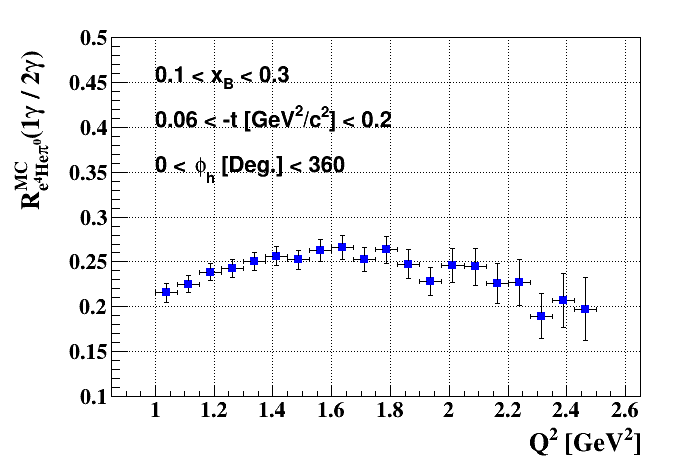
\includegraphics[scale=0.30]{fig_dvcs/e4Hegamma_e4Hepi0_Q2.png}
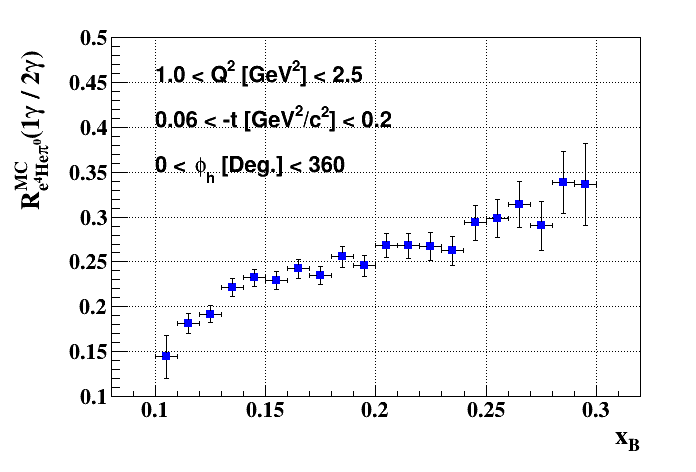
\includegraphics[scale=0.30]{fig_dvcs/e4Hegamma_e4Hepi0_xB.png}
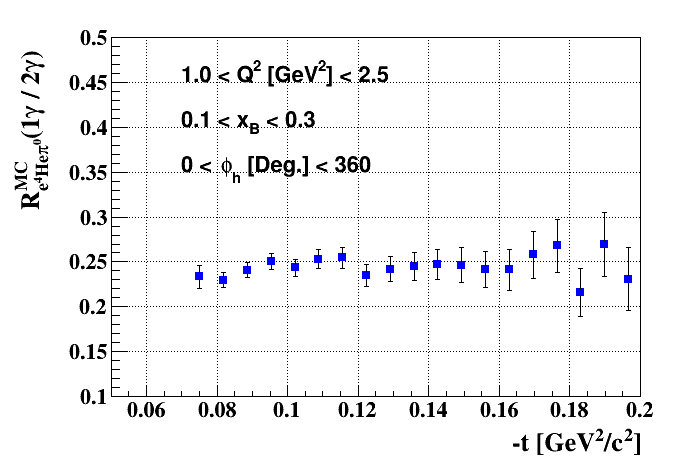
\includegraphics[scale=0.30]{fig_dvcs/e4Hegamma_e4Hepi0_t.png}
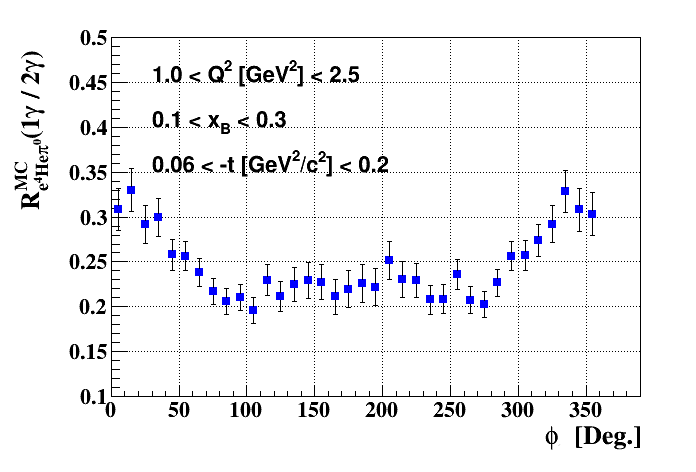
\includegraphics[scale=0.30]{fig_dvcs/e4Hegamma_e4Hepi0_Phi.png}
\caption{The coherent channel acceptance ratios as a function of the kinematic 
variables: $Q^{2}$ (top left), $x_{B}$ (top right), $-t$ (bottom left), and 
$\phi$ (bottom right). }
\label{fig:coh_acceptance _ratios}
\end{figure}

\begin{figure}[tpb]
\centering
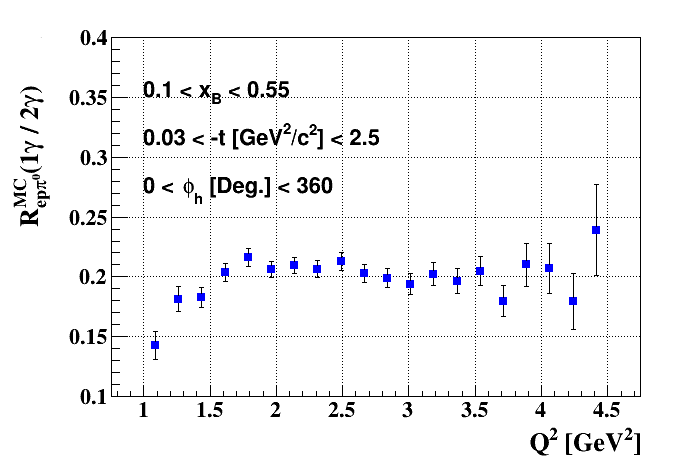
\includegraphics[scale=0.30]{fig_dvcs/epgamma_eppi0_Q2.png}
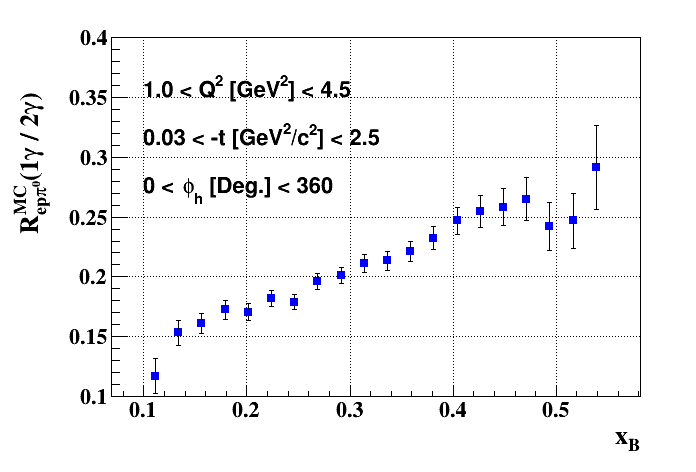
\includegraphics[scale=0.30]{fig_dvcs/epgamma_eppi0_xB.png}
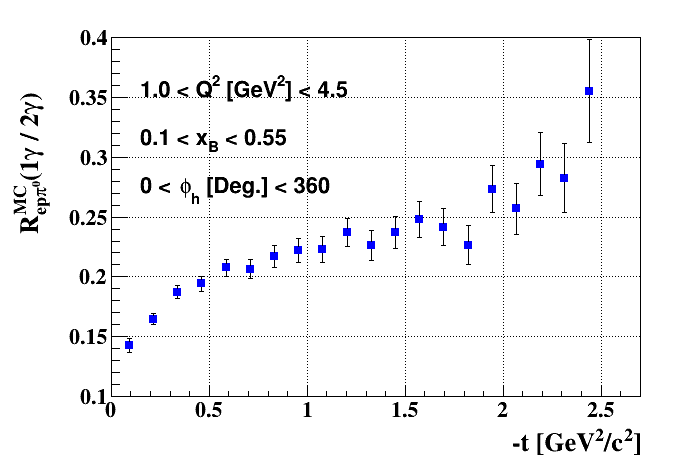
\includegraphics[scale=0.30]{fig_dvcs/epgamma_eppi0_t.png}
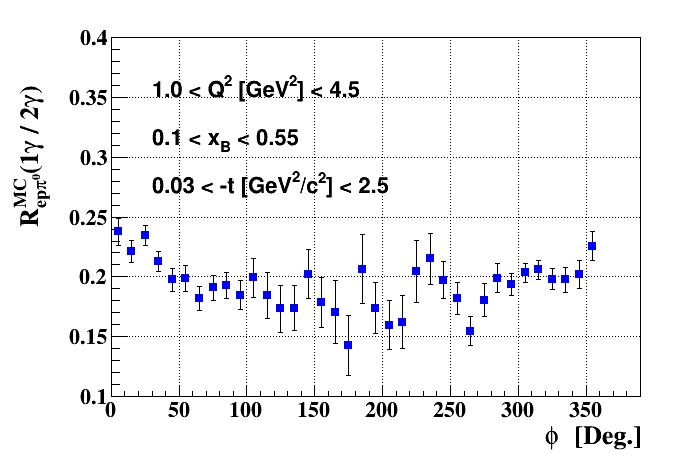
\includegraphics[scale=0.30]{fig_dvcs/epgamma_eppi0_Phi.png}
\caption{The incoherent channel acceptance ratios as a function of the 
kinematic variables: $Q^{2}$ (top left), $x_{B}$ (top right), $-t$ (bottom 
left), and $\phi$ (bottom right).}
\label{fig:incoh_acceptance _ratios}
\end{figure}

\begin{figure}[tpb]
\includegraphics[scale=0.4]{fig_updated/T_ratio_pi0_dvcs_Coh_t.pdf}
\includegraphics[scale=0.4]{fig_updated/T_ratio_pi0_dvcs_InCoh_t.pdf}
\caption{The experimental coherent (left) and incoherent (right) $\pi^{0}$ 
contamination with respect to the experimental DVCS events as a function of the 
transfered momentum squared -$t$. The data is integrated over the kinematical 
variables $Q^2$, $x_B$, and $\phi$.  }
\label{fig:cont_yield}
\end{figure}





As presented in the previous section, we construct two-dimensional bins: 
$Q^2$-$\phi$, $x_B$-$\phi$ and -$t$-$\phi$. Thus, for each bin in $Q^2$, $x_B$ 
and $-t$, we assume that the acceptance ratio does not change a lot within the 
bin range and we construct the one-dimensional acceptance ratio as a function 
of $\phi$. We also carried out four-dimensional background subtraction, in 
which the acceptance ratio has been extracted from simulation as a function of 
$Q^2$, $x_B$, -$t$, and $\phi$. The difference between the reconstructed 
beam-spin asymmetries using two-dimensional and four-dimensional background 
subtraction are presented in figures \ref{fig:coh_binning} and 
\ref{fig:incoh_binning} for the coherent and the incoherent DVCS channels.  
Even though the two-dimensional subtraction is a good approximation, a 
four-dimensional subtraction is applied on the final results presented next 
chapter. 

\begin{figure}[tbp]
   \centering
    \includegraphics[height=6.0cm]{fig_rtpc/updates/BSA_Coherent_xB.png}
    \includegraphics[height=6.0cm]{fig_rtpc/updates/diff_BSA_Coherent_xB_2.png}
    \caption{On top: the reconstruct coherent beam-spin asymmetries as a 
    function of $\phi$ in $x_{B}$ bins using two-dimensional (in blue) and 
 four-dimensional (in green) background subtraction.  On bottom: the difference 
 between the two asymmetries as a function of $\phi$.}
    \label{fig:coh_binning}
    \end{figure}            

    \begin{figure}[tbp]
       \centering
    \includegraphics[height=5.2cm]{fig_rtpc/updates/BSA_InCoherent_xB.png}
    \includegraphics[height=5.2cm]{fig_rtpc/updates/diff_BSA_InCoherent_xB_2.png}
    \caption{On top: the reconstruct incoherent beam-spin asymmetries using    
    two-dimensional (in blue) and four-dimensional (in green) background 
 subtraction.  On bottom: the difference between the two asymmetries as a 
 function of $\phi$.}
    \label{fig:incoh_binning}
    \end{figure}                                                                  

  
Regarding other backgrounds, the procedures carried out in this work followed 
the same guidelines as for DVCS analysis on the nucleon. The neutral pion 
production occurs "without threshold" as seen from the $eHe\gamma$ sample, 
meaning that the contamination from $eHe\pi^0$ with one photon lost is 
distributed all the way down to the DVCS, in the limit where the second photon 
energy becomes negligible in the lab. Single charged pion production occurs 
with a small threshold but is inconsistent with the already detected particles 
($e$ and $^{4}$He). Two pion production is entirely cleaned up by the 
exclusivity cuts. Scattering from the windows is excluded by the vertex cuts.  
As far as accidental, we correct for that as presented in the following 
section.   


\subsection{Accidental contaminations}


The $\Delta z$ distributions between the recoil hadrons and the scattered 
electrons, see figures \ref{fig:rtpc_delta_z} and 
\ref{fig:proton_delta_z_e_prot}, indicate that accidental background events are 
contributing inside the exclusive DVCS. In order to estimate and correct 
this background contribution, we processed our dataset with the previously 
presented exclusive requirements without any constraints on the z-vertex of the 
final state particle nor on the correspondence between them, $\Delta z$. The 
results for the identified coherent DVCS events are presented in figure 
\ref{fig:delta_z_after_ex}. This guides us to correct for these accidentals in 
our asymmetries in the form: $ A_{LU~~corr.} = \frac{1}{1 - contamination} 
A_{LU}$, with a 4.1$\%$ global accidental contamination for the coherent DVCS 
channel (see numbers in table~\ref{table:Events_numbers}). The same procedures 
were performed on the incoherent channel, and a 
global contamination of 6.5$\%$ has been observed.

\begin{figure}[tbp]
\centering
\includegraphics[height=7.2cm]{fig_dvcs/rtpc_delta_z_acc.png}
\caption{The z-vertex correspondence between the scattered electron and the 
   recoil $^{4}He$ for the identified coherent DVCS events after the 
   exclusivity cuts in the two modules of the RTPC separately without any 
   initial constrains on z-vertices of the individual particles.  Table 
\ref{table:Events_numbers} summarizes the cut numerically.}
\label{fig:delta_z_after_ex}
 \end{figure}

\begin{table}[!h]
   \centering
   \begin{center}
      \begin{tabular}{|l|l|l|}
         \hline
         \multicolumn{3}{ |c| }{Number of coherent DVCS events} \\
         \hline
         $\Delta z$ [mm] & Left module & Right module\\
         \hline
         [-50:-30] & 42 & 77 \\
         \hline
         [-20:20]  & 2741 & 2856\\
         \hline
         [30:50]   & 34 &  78 \\
         \hline
         Contamination percentage  & 2.7$\%$  & 5.4$\%$ \\
         \hline 
      \end{tabular}
      \caption{The numbers of the identified coherent DVCS events in the 
      different regions in $\Delta z$ for the two modules of the RTPC.}
      \label{table:Events_numbers}
   \end{center}
\end{table}



~\newpage
\section{Statistical uncertainties}
In terms of the collected number of events in each beam-helicity state ($N^{+}$, $N^{-}$), $A_{LU}$ can be expressed as:
\begin{equation}
A_{LU} = \frac{1}{P_{B}} \frac{N^{+} - N^{-}}{N^{+} + N^{-} }.
\label{equation: ALU}
\end{equation}
where $P_{B}$ is the beam polarization, $N^{+}$ and $N^{-}$ are the background-subtracted yields of DVCS events. The statistical uncertainties on the measured $A_{LU}$ can be derived as:
\begin{equation}
\Delta A = \frac{1}{P_{B}} \sqrt{\left(\frac{\partial A}{\partial N^{+}}\right)^{2} (\Delta N^{+})^{2} + \left(\frac{\partial A}{\partial N^{-}}\right)^{2} (\Delta N^{-})^{2}} = \frac{1}{P_{B}} \sqrt{\frac{(2N^{-} \Delta N^{+})^{2} + (2N^{-} \Delta N^{+})^{2}}{(N^{+} + N^{-})^{4} }},
\end{equation}
where $N^{+}$ and $N^{-}$ are
\begin{equation}
N^{\pm} = N^{\pm}_{e^{4}He\gamma} - R ~ N^{\pm}_{e^{4}He\pi^{0}},
\end{equation} 
and $R$ is the calculated background acceptance ratio from the simulation. The statistical uncertainty on the counts ($N^{\pm}$) is
\begin{equation}
(\Delta N^{\pm})^{2} = (\Delta N^{\pm}_{e^{4}He\gamma})^{2} + (R ~ \Delta N^{\pm}_{e^{4}He\pi^{0}})^{2} 
                       =  N^{\pm}_{e^{4}He\gamma} + R^2 N^{\pm}_{e^{4}He\pi^{0}}. 
\end{equation}
The errors on $P_{B}$ and $R$ are not considered statistical errors. They contribute in the systematic uncertainties, as will be discussed in the following section. This derivation is valid for the coherent and the incoherent DVCS channels.



\section{Systematic uncertainties}

It is particularly convenient to use the $A_{LU}$ as a DVCS observable, 
because most of the experimental systematic uncertainties, such as 
normalization and efficiencies that appear in the cross sections cancel out in 
the asymmetry ratio. However, some sources still affect this asymmetry and 
contribute in the systematic uncertainties on the measured $A_{LU}$. The main 
known sources of systematic errors are: the DVCS selection cuts, the fitting 
sensitivity to our binning, the beam polarization, the background acceptance 
ratio and the radiative corrections. In the following, we present an estimation 
of the contribution from each source.  

 

\paragraph{DVCS selection cuts} ~\\
In order to evaluate the systematic uncertainties stemming from the DVCS 
selection cuts, the analysis was repeated changing cuts. As it can be seen in 
figure \ref{fig:coh_exclusivty_cuts}, the 3$\sigma$ cuts cover up to 97$\%$ of 
the events in all the distributions except the $e^{4}He\gamma$ missing mass 
distribution. In order to investigate the effect of taking different cuts on 
the reconstructed $A_{LU}$, we fix the 3$\sigma$ cuts on all the exclusive 
quantities except for the cut on $e^{4}He\gamma$ missing mass. For the 
incoherent channel, the same procedure is carried out on the $ep\gamma$ missing 
mass distribution. The results can be seen in figure 
\ref{fig:cuts_e4Hegamma_M2_Mis}. The maximum variation that has been observed 
on the $A_{LU}$ observable between 3$\sigma$ cut and the other cuts 
($\frac{\Delta A^{sys. cuts}_{LU}}{A_{LU}}$) is equal to  8$\%$ for the 
coherent channel and to 6$\%$ for the incoherent channel at $\phi = 90^{\circ}$ 
extracted from a fit, in the form of $\frac{\alpha sin(\phi)}{1+\beta cos(\phi) 
+ \eta cos(2\phi)}$, to $A_{LU}(\phi)$ distribution. The fit parameters are 
plotted as functions of the cut widths in figures \ref{fig:sys_fit_alpha} to 
\ref{fig:sys_fit_Alu}.

\begin{figure}[h!]
\includegraphics[scale=0.31]{fig_dvcs/e4Hegamma_M2_Mis_sig.png}
\includegraphics[scale=0.31]{fig_dvcs/epgamma_M2_Mis_sig.png}
\includegraphics[scale=0.31]{fig_dvcs/e4Hegamma_e4Hepi0_Phi_2.png}
\hspace{-0.2in}\includegraphics[scale=0.31]{fig_dvcs/R_epgamma_eppi0_Phi.png}
\includegraphics[scale=0.31]{fig_dvcs/BSA_Coherent_sigmas.png}
\includegraphics[scale=0.31]{fig_dvcs/BSA_InCoherent_sigmas.png}
\caption{The systematic uncertainties stemming from the DVCS selection cuts in 
the coherent (left column) and the incoherent (right column) channels. On the 
top: the missing mass squared of $e^{4}He\gamma$ and $ep\gamma$. The different 
vertical coloured lines indicate the different cuts: 1$\sigma$, 2$\sigma$, ...  
5$\sigma$. In the middle: the coherent (incoherent) acceptance ratios versus 
$\phi$ for the different configurations of the cuts. On the bottom: the 
reconstructed $A_{LU}$ as a function of $\phi_{h}$ for the different cut 
widths.}
\label{fig:cuts_e4Hegamma_M2_Mis}
\end{figure}

\begin{figure}[tbp]
 \includegraphics[height=6.2cm]{fig_dvcs/coh_alpha_Nsig.png}
    \includegraphics[height=6.2cm]{fig_dvcs/incoh_alpha_Nsig.png}
       \caption{The coherent (left) and incoherent (right) $\alpha$ parameter 
          of
       the fits as a function of cut width.  }
       \label{fig:sys_fit_alpha}
    \end{figure}

\begin{figure}[tbp]
      \includegraphics[height=6.2cm]{fig_dvcs/coh_beta_Nsig.png}
         \includegraphics[height=6.2cm]{fig_dvcs/incoh_beta_Nsig.png}
            \caption{The coherent (left) and incoherent (right) $\beta$ 
               parameter of the
            fits as a function of cut width.  }
            \label{fig:sys_fit_beta}
         \end{figure}

\begin{figure}[tbp]
\includegraphics[height=6.2cm]{fig_dvcs/coh_eta_Nsig.png}
\includegraphics[height=6.2cm]{fig_dvcs/incoh_eta_Nsig.png}
   \caption{The coherent (left) and incoherent (right) $\eta$ parameter of the
   fits as a function of cut width.  }
   \label{fig:sys_fit_eta}
\end{figure}

\begin{figure}[tbp]
\includegraphics[height=6.2cm]{fig_dvcs/coh_chi2_Nsig.png}
\includegraphics[height=6.2cm]{fig_dvcs/incoh_chi2_Nsig.png}
   \caption{The coherent (left) and incoherent (right) $\chi^{2}$ parameter of
   the fits as a function of cut width.}
   \label{fig:sys_fit_chi2}
\end{figure}

 
\begin{figure}[tbp]
\includegraphics[height=6.2cm]{fig_dvcs/coh_Alu_Nsig.png}
\includegraphics[height=6.2cm]{fig_dvcs/incoh_Alu_Nsig.png}
   \caption{The coherent (left) and incoherent (right) 
      beam-spin asymmetry at
   $\phi = 90 ^{\circ}$. }
   \label{fig:sys_fit_Alu}
\end{figure}



\paragraph{Fitting sensitivity to our binning} ~\\
In order to evaluate how sensitive are the fit results to our binning, we 
binned the data into 11 bins in $\phi$ and we compared the reconstructed 
asymmetries to the results from our 9 binning. Figure 
\ref{fig:coh_bins_phi_9_11} shows the coherent reconstructed $A_{LU}$ as a 
function of $\phi$ in $Q^{2}$, $x_B$ and $-t$ bins.  The coherent, figure 
\ref{fig:coh_BSA_9_11}, and the incoherent, figure \ref{fig:incoh_BSA_9_11}, 
measured $A_{LU}$ at $\phi = 90 ^{\circ}$ are showing an overall average of 
5.1$\%$ and 7.1$\%$ systematic uncertainties respectively, which will be added 
to our estimated uncertainties for the extracted asymmetries at $\phi = 
90^{\circ}$.



\begin{figure}[tbp]
   \centering
      \includegraphics[height=6.2cm]{fig_dvcs/sBSA_Coherent_Q2.png}
      \includegraphics[height=6.2cm]{fig_dvcs/sBSA_Coherent_xB.png}
      \includegraphics[height=6.2cm]{fig_dvcs/sBSA_Coherent_t.png}
     \caption{The measured coherent beam-spin asymmetry as
     a function of $\phi$ in $Q^{2}$, $x_B$ and $-t$ bins, using two binning 
  sets in $\phi$: 9 bins (in blue) and 11 bins (in red).}
      \label{fig:coh_bins_phi_9_11}
    \end{figure}

\begin{figure}[tbp]
   \centering
      \includegraphics[height=9.2cm]{fig_dvcs/BSA_Coherent_9_11.png}
      \caption{The coherent $A_{LU}$($\phi = 90 ^{\circ}$), from the fit, as a 
      function of $Q^{2}$, $x_B$ and $-t$, using 9 (in blue) and 11 (in red) 
   bins in $\phi$.}
      \label{fig:coh_BSA_9_11}
    \end{figure}

\begin{figure}[tbp]
   \centering
      \includegraphics[height=9.2cm]{fig_dvcs/BSA_InCoherent_9_11.png}
      \caption{The incoherent $A_{LU}$($\phi = 90 ^{\circ}$), from the fit, as 
         a function of $Q^{2}$, $x_B$ and $-t$, using 9 (in blue) and 11 (in 
      red) bins in $\phi$. }
      \label{fig:incoh_BSA_9_11}
    \end{figure}

\paragraph{Beam polarization} ~\\
The beam polarization has been measured regularly during the CLAS-EG6 data 
taking period by using the Hall B M\o ller polarimeter. This polarimeter 
measures the angular distribution of the M\o ller electrons to obtain the beam 
polarization. Figure \ref{fig:beam_polarization} shows the M\o ller 
measurements taken during the EG6 experiment. A linear fit to these 
measurements yields a mean polarization value of 0.8367. The precision of the 
Hall B M\o ller polarimeter ($\frac{\Delta P}{P})$ was measured to be around 
3.5$\%$ \cite{hallb_polarimeter}. We asume therefore a 3.5$\%$ systematic 
uncertainty on the measured asymmetries ($\frac{\Delta A^{sys.  
p}_{LU}}{A_{LU}}$~=~$\frac{\Delta P}{P}$).

\begin{figure}[tp]
\centering
\includegraphics[scale=0.25]{fig_dvcs/beam_polarization.png}
\caption{Beam polarization measurements during the CLAS-EG6 running period.  
The red squares are the measurements with a negative current in the Helmholtz 
coils of the M\o ller polarimeter and the purple triangles are these with a 
positive current. The figure is taken from \cite{yohann}.} 
\label{fig:beam_polarization}
\end{figure}


\paragraph{Acceptance ratio} ~\\
Predominantly, two techniques are used to estimate the systematic uncertainty 
associated with the calculated acceptance ratio (R). The first is via repeating 
the analysis by implementing R differently, while the second technique is by 
using two generating models to calculate R.

Both methods were investigated in this work. Regarding the first method, the 
analysis was repeated by taking three different values for R: 0.8*R, R and 
1.2*R. The beam-spin asymmetries at $\phi = 90^{\circ}$ were extracted and 
compared, see figure \ref{fig:background_sub_sys_uncer}. A maximum variation of 
2$\%$ (0.6$\%$) has been observed on the incoherent (coherent) $A_{LU}$ at 
$\phi = 90^{\circ}$. 

\begin{figure}[tp]
\includegraphics[scale=0.30]{fig_dvcs/final_coh_BSA_NR.png}
\includegraphics[scale=0.30]{fig_dvcs/final_incoh_BSA_NR.png}
\caption{The extracted beam-spin asymmetries at $\phi = 90^{\circ}$ as a 
function of three sets of the calculated acceptance ratios: 0.8*R, 1.0*R and 
1.2*R, for the coherent (on the left) and the incoherent (on the right) DVCS 
channels.} \label{fig:background_sub_sys_uncer}
\end{figure}

For the second technique, in fact there is only one event generator available, 
presented in section \ref{Event_generator}. Nevertheless, one can still use 
this method by generating events with or without the cross section 
parametrization. In the absence of the parametrization, the generated events 
are flat in the four kinematic variables ($Q^2$, $-t$, $x_B$, $\phi$). The 
calculated coherent and incoherent acceptance ratios (R) with and without the 
cross section parametrization are shown in figure 
\ref{fig:accep_ratio_sys_uncer}. One can see that the difference between the 
calculated acceptance ratios is almost constant. Thus, we can conclude that the 
first method of taking $\pm$20$\%$ on R is is an adequate way to obtain an 
estimation of the systematic uncertainty associated to the calculated 
acceptance ratios.
\begin{figure}[h!]
\includegraphics[scale=0.34]{fig_results/coh_accp_ratio_phi.png}
\includegraphics[scale=0.34]{fig_results/incoh_accp_ratio_phi.png}
\caption{The coherent (on the left) and the incoherent (on the right) 
acceptance ratios ($R$) as function of the angle $\phi$. In both plots, the 
blue (red) points are the ratios with (without) the cross section 
parametrization.} \label{fig:accep_ratio_sys_uncer}
\end{figure}

\paragraph{Radiative corrections} ~\\
In this analysis, we have assumed that the beam-spin asymmetry arises from the 
leading twist DVCS amplitude and its interference with the BH process.  
However, there are higher-order electromagnetic corrections which can affect 
the beam-spin asymmetry. Andrei V. Afanasev and his collaborators have 
estimated the corrections to $A_{LU}$ which arise from such effects in a 
model-independent way \cite{Afanasev}. They have performed one-loop corrections 
on the outgoing electron as only the radiation from it affects the $A_{LU}$.  
They found that the correction does not exceed 0.1$\%$ at a 4.25 GeV electron 
beam energy and Q$^{2}$=1.25 GeV$^{2}$. In our case, as the radiative emission 
is inversely proportional to the mass of the radiating particle, the helium and 
the proton contributions are negligible compared to the leptonic one.  
Therefore, we can still take the result of Afanasev as a good estimation for 
the radiative  effects on our measured $A_{LU}$.

%\paragraph{Beam asymmetry}
%The injector of JLab produces electrons with positive and negative helicities 
%in equal %time in principle. To ensure this equality between the two helicity 
%configurations., %figure \ref{fig:beam_charge} shows the deposited charge 
%ratio of the positive helicity %electrons to the negative ones in the 
%individual runs. A 2$\%$  maximum deviation from %one. Thus, the integrated 
%beam charge ratio induces 1.1$\%$ systematic uncertainty to %$A_{LU}$ on both 
%DVCS channels.\\
%\begin{figure}[h!]
%\hspace{-0.3in}
%\includegraphics[scale=0.4]{fig_bsa/qplus_qminus_RunNum.png}
%\caption{The beam charge ratio between the positive and the negative helicites.} 
%\label{fig:beam_charge}


\paragraph{Systematic uncertainty summary} ~\\
The total systematic uncertainty is the quadratic sum of the previously 
described individual uncertainties. Table \ref{Table:systematic_uncertainties} 
summarizes the sources of systematic uncertainty and their contributions on the 
measured $A_{LU}$ at $\phi = 90^{\circ}$, that will be added quadratically to 
the statistical uncertainties on $A_{LU}$. 

\begin {table}[!h]
\begin{center}
\begin{tabular}{|l|c|c|c|}
\hline
\bf Systematic source & \bf  Coherent channel  & \bf Incoherent channel & \bf Type of systematic 
error\\
\hline
DVCS cuts & 8 $\%$ &  6 $\%$ & bin to bin\\
\hline
Data binning & 5.1$\%$ & 7.1$\%$ &bin to bin\\
\hline
Beam polarization &  3.5$\%$ &  3.5$\%$& Normalization\\
\hline
Acceptance ratio &  0.6$\%$ &  2.0$\%$ &bin to bin\\
\hline
%Beam charge asymmetry &  ~~~~~1.1$\%$&  ~~~~~1.1$\%$\\
%\hline
Radiative corrections &  0.1$\%$ & 0.1$\%$ & bin to bin\\
\hline
\textbf{Total} &  \textbf{10.1}$\%$ &   \textbf{10.1}$\%$ &bin to 
bin\\
\hline
\end{tabular}
\caption{The systematic uncertainties on the measured coherent and incoherent 
beam-spin asymmetries at $\phi = 90^{\circ}$.}
\label{Table:systematic_uncertainties}
\end{center}
\end{table}

In addition to evaluating the systematic uncertainties on $A_{LU}$ at $\phi = 
90^{\circ}$, we performed bin by bin, in $\phi$, extraction of these 
uncertainties. For instance, regarding the bin extraction from the source 'data 
binning' listed in table \ref{Table:systematic_uncertainties}, the uncertainty 
is calculated as the difference between the two reconstructed asymmetries.  
Similar procedures have been carried out for the other studies, and finally all 
the contributions were added quadratically. These systematic uncertainties will 
be shown with the final asymmetry results in the following chapter.  
